%%%%%%%%%%%%%%%%%%%%%%%%%%%%%%%%%%%%%%%%%
% Beamer Presentation
% LaTeX Template
% Version 2.0 (March 8, 2022)
%
% This template originates from:
% https://www.LaTeXTemplates.com
%
% Author:
% Vel (vel@latextemplates.com)
%
% License:
% CC BY-NC-SA 4.0 (https://creativecommons.org/licenses/by-nc-sa/4.0/)
%
%%%%%%%%%%%%%%%%%%%%%%%%%%%%%%%%%%%%%%%%%

%----------------------------------------------------------------------------------------
%	PACKAGES AND OTHER DOCUMENT CONFIGURATIONS
%----------------------------------------------------------------------------------------

\documentclass[
	11pt, % Set the default font size, options include: 8pt, 9pt, 10pt, 11pt, 12pt, 14pt, 17pt, 20pt
	%t, % Uncomment to vertically align all slide content to the top of the slide, rather than the default centered
	%aspectratio=169, % Uncomment to set the aspect ratio to a 16:9 ratio which matches the aspect ratio of 1080p and 4K screens and projectors
]{beamer}

\graphicspath{{Images/}{./}} % Specifies where to look for included images (trailing slash required)

\usepackage{booktabs} % Allows the use of \toprule, \midrule and \bottomrule for better rules in tables

\usepackage{siunitx}
\usepackage{tikz}
\usetikzlibrary{arrows.meta}
\usetikzlibrary{patterns}
%----------------------------------------------------------------------------------------
%	SELECT LAYOUT THEME
%----------------------------------------------------------------------------------------

% Beamer comes with a number of default layout themes which change the colors and layouts of slides. Below is a list of all themes available, uncomment each in turn to see what they look like.

%\usetheme{default}
%\usetheme{AnnArbor}
%\usetheme{Antibes}
%\usetheme{Bergen}
%\usetheme{Berkeley}
%\usetheme{Berlin}
%\usetheme{Boadilla}
%\usetheme{CambridgeUS}
%\usetheme{Copenhagen}
%\usetheme{Darmstadt}
%\usetheme{Dresden}
%\usetheme{Frankfurt}
%\usetheme{Goettingen}
%\usetheme{Hannover}
%\usetheme{Ilmenau}
%\usetheme{JuanLesPins}
%\usetheme{Luebeck}
\usetheme{Madrid}
%\usetheme{Malmoe}
%\usetheme{Marburg}
%\usetheme{Montpellier}
%\usetheme{PaloAlto}
%\usetheme{Pittsburgh}
%\usetheme{Rochester}
%\usetheme{Singapore}
%\usetheme{Szeged}
%\usetheme{Warsaw}

%----------------------------------------------------------------------------------------
%	SELECT COLOR THEME
%----------------------------------------------------------------------------------------

% Beamer comes with a number of color themes that can be applied to any layout theme to change its colors. Uncomment each of these in turn to see how they change the colors of your selected layout theme.

%\usecolortheme{albatross}
%\usecolortheme{beaver}
%\usecolortheme{beetle}
%\usecolortheme{crane}
%\usecolortheme{dolphin}
%\usecolortheme{dove}
%\usecolortheme{fly}
%\usecolortheme{lily}
%\usecolortheme{monarca}
%\usecolortheme{seagull}
%\usecolortheme{seahorse}
%\usecolortheme{spruce}
%\usecolortheme{whale}
%\usecolortheme{wolverine}

%----------------------------------------------------------------------------------------
%	SELECT FONT THEME & FONTS
%----------------------------------------------------------------------------------------

% Beamer comes with several font themes to easily change the fonts used in various parts of the presentation. Review the comments beside each one to decide if you would like to use it. Note that additional options can be specified for several of these font themes, consult the beamer documentation for more information.

\usefonttheme{default} % Typeset using the default sans serif font
%\usefonttheme{serif} % Typeset using the default serif font (make sure a sans font isn't being set as the default font if you use this option!)
%\usefonttheme{structurebold} % Typeset important structure text (titles, headlines, footlines, sidebar, etc) in bold
%\usefonttheme{structureitalicserif} % Typeset important structure text (titles, headlines, footlines, sidebar, etc) in italic serif
%\usefonttheme{structuresmallcapsserif} % Typeset important structure text (titles, headlines, footlines, sidebar, etc) in small caps serif

%------------------------------------------------

%\usepackage{mathptmx} % Use the Times font for serif text
\usepackage{palatino} % Use the Palatino font for serif text

%\usepackage{helvet} % Use the Helvetica font for sans serif text
\usepackage[default]{opensans} % Use the Open Sans font for sans serif text
%\usepackage[default]{FiraSans} % Use the Fira Sans font for sans serif text
%\usepackage[default]{lato} % Use the Lato font for sans serif text

%----------------------------------------------------------------------------------------
%	SELECT INNER THEME
%----------------------------------------------------------------------------------------

% Inner themes change the styling of internal slide elements, for example: bullet points, blocks, bibliography entries, title pages, theorems, etc. Uncomment each theme in turn to see what changes it makes to your presentation.

%\useinnertheme{default}
\useinnertheme{circles}
%\useinnertheme{rectangles}
%\useinnertheme{rounded}
%\useinnertheme{inmargin}

%----------------------------------------------------------------------------------------
%	SELECT OUTER THEME
%----------------------------------------------------------------------------------------

% Outer themes change the overall layout of slides, such as: header and footer lines, sidebars and slide titles. Uncomment each theme in turn to see what changes it makes to your presentation.

%\useoutertheme{default}
%\useoutertheme{infolines}
%\useoutertheme{miniframes}
%\useoutertheme{smoothbars}
%\useoutertheme{sidebar}
%\useoutertheme{split}
%\useoutertheme{shadow}
%\useoutertheme{tree}
%\useoutertheme{smoothtree}

%\setbeamertemplate{footline} % Uncomment this line to remove the footer line in all slides
%\setbeamertemplate{footline}[page number] % Uncomment this line to replace the footer line in all slides with a simple slide count

%\setbeamertemplate{navigation symbols}{} % Uncomment this line to remove the navigation symbols from the bottom of all slides

%----------------------------------------------------------------------------------------
%	PRESENTATION INFORMATION
%----------------------------------------------------------------------------------------

\title[]{Analýza vazby mezi teplotou vzduchu ve standardní výšce a v hladině bylinného patra v závislosti na meteorologických podmínkách} % The short title in the optional parameter appears at the bottom of every slide, the full title in the main parameter is only on the title page

\author[]{Vojtěch Klimeš} % Presenter name(s), the optional parameter can contain a shortened version to appear on the bottom of every slide, while the main parameter will appear on the title slide

\institute[MFF UK]{Univerzita Karlova} % Your institution, the optional parameter can be used for the institution shorthand and will appear on the bottom of every slide after author names, while the required parameter is used on the title slide and can include your email address or additional information on separate lines

\date[12.4.2023]{Seminář KFA} % Presentation date or conference/meeting name, the optional parameter can contain a shortened version to appear on the bottom of every slide, while the required parameter value is output to the title slide

%----------------------------------------------------------------------------------------

\begin{document}

%----------------------------------------------------------------------------------------
%	TITLE SLIDE
%----------------------------------------------------------------------------------------

\begin{frame}
	\titlepage % Output the title slide, automatically created using the text entered in the PRESENTATION INFORMATION block above
\end{frame}

%----------------------------------------------------------------------------------------
%	TABLE OF CONTENTS SLIDE
%----------------------------------------------------------------------------------------

% The table of contents outputs the sections and subsections that appear in your presentation, specified with the standard \section and \subsection commands. You may either display all sections and subsections on one slide with \tableofcontents, or display each section at a time on subsequent slides with \tableofcontents[pausesections]. The latter is useful if you want to step through each section and mention what you will discuss.

\begin{frame}
	\frametitle{Obsah prezentace} % Slide title, remove this command for no title
	
	\tableofcontents % Output the table of contents (all sections on one slide)
	%\tableofcontents[pausesections] % Output the table of contents (break sections up across separate slides)
\end{frame}

%----------------------------------------------------------------------------------------
%	PRESENTATION BODY SLIDES
%----------------------------------------------------------------------------------------

\section{Úvod} % Sections are added in order to organize your presentation into discrete blocks, all sections and subsections are automatically output to the table of contents as an overview of the talk but NOT output in the presentation as separate slides

%------------------------------------------------

\subsection{Problematika}

\begin{frame}
	\frametitle{Problematika}
	\begin{itemize}
		\item Teplota a jiné meteorologické podmínky jsou typicky měřeny standardizovanými meteorologickými stanicemi.
		\item Teploty v $\SI{2}{m}$ nereflektují podmínky, v kterých žije většina organismů
		\item Lesní mikroklima je velmi odlišné od klimatu v okolí meteorologické stanice.
	\end{itemize}
\end{frame}

\begin{frame}
	\frametitle{Problematika}
	\begin{figure}
		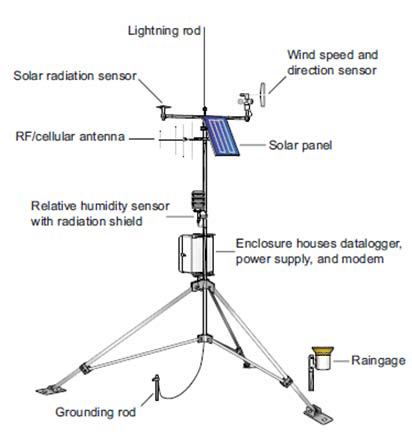
\includegraphics[width=0.6\linewidth]{meteo_station.png}
		\caption{Příklad automatické stanice}
	\end{figure}
\end{frame}

\begin{frame}
	\frametitle{Problematika}
	Cílem této bakalářské práce je prozkoumat a vysvětlit rozdíl mezi teplotou naměřenou v lese v Šumavském Národním parku ve $\SI{2}{m}$ a teplotou při zemi pomocí meteorologických podmínek naměřených na nejbližších stanicích.
	\bigskip

	Faktory, které mají vliv na naměřené teploty rozdělíme do následujících skupin: topografické a vegetační.
\end{frame}

\subsection{Klima nízko nad zemí}
\begin{frame}
	\frametitle{Klima nízko nad zemí}
\begin{figure}
\centering
	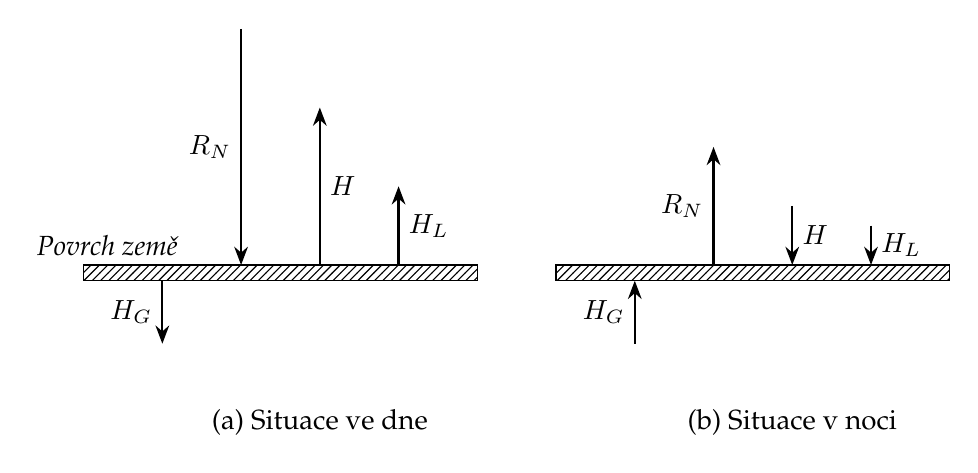
\begin{tikzpicture}
  % Part a: Day
  \draw (-1,0) -- (4,0);
  \draw[pattern=north east lines] (-1,0) rectangle (4,-0.2);
	\draw[-{Stealth},thick] (1,3) -- (1,0) node[midway,left] {$R_N$};
  \draw[-{Stealth},thick] (2,0) -- (2,2) node[midway,right] {$H$};
  \draw[-{Stealth},thick] (3,0) -- (3,1) node[midway,right] {$H_L$};
  \draw[-{Stealth},thick] (0,-0.2) -- (0,-1) node[midway,left] {$H_G$};
  \node at (2,-2) {(a) Situace ve dne};
	\node at (-0.7,0.25) {\textit{Povrch země}};

  % Part b: Night
  \begin{scope}[xshift=6cm]
    \draw (-1,0) -- (4,0);
    \draw[pattern=north east lines] (-1,0) rectangle (4,-0.2);
    \draw[-{Stealth},thick] (1,0) -- (1,1.5) node[midway,left] {$R_N$};
    \draw[-{Stealth},thick] (2,0.75) -- (2,0) node[midway,right] {$H$};
    \draw[-{Stealth},thick] (3,0.5) -- (3,0) node[midway,right] {$H_L$};
    \draw[-{Stealth},thick] (0,-1) -- (0,-0.2) node[midway,left] {$H_G$};
    \node at (2,-2) {(b) Situace v noci};
  \end{scope}
	\end{tikzpicture}
	\caption{Schéma ukazující rozdíl mezi tokem tepla v noci a přes den}
\label{fig:schema}
\end{figure}
\end{frame}

\begin{frame}
	\frametitle{Klima nízko nad zemí}
	\begin{itemize}
		\item Teplota dosahuje maxima 1 až 2 hodiny po maximální insolaci, minima v brzkých ranních hodinách.
		\item Teplotní gradienty v blízkosti vyhřátého povrchu může dosáhnout až hodnot $\SI{20}{K\ mm^{-1}}$. Teplotní rozdíly mezi dnem a nocí jsou v blízkosti povrchu větší.
	\end{itemize}
\end{frame}

\subsection{Topografie a vegetace}
%------------------------------------------------

\begin{frame}
	\frametitle{Topografie a struktura krajiny}
	
	\begin{itemize}
		\item Okraj lesa
		\item Sklon svahu
		\item Nadmořská výška
		\item Údolí/hřeben
	\end{itemize}
	
	\bigskip % Vertical whitespace
	
\end{frame}

\begin{frame}
	\frametitle{Vegetace}
	\begin{itemize}
		\item Albedo
		\item Tok tepla
		\item Rychlost větru
		\item Vlhkost vzduchu
		\item Srážky
	\end{itemize}
\end{frame}

%------------------------------------------------

\subsection{Data z ČHMÚ}

\begin{frame}
	\frametitle{Data z ČHMÚ}
	Stanice: Kvilda, Horská Kvilda, Churáňov, Borová Lada, Javoří Pila

	Maximální časový interval: 12.10.2019 - 19.5.2021
	\begin{figure}
		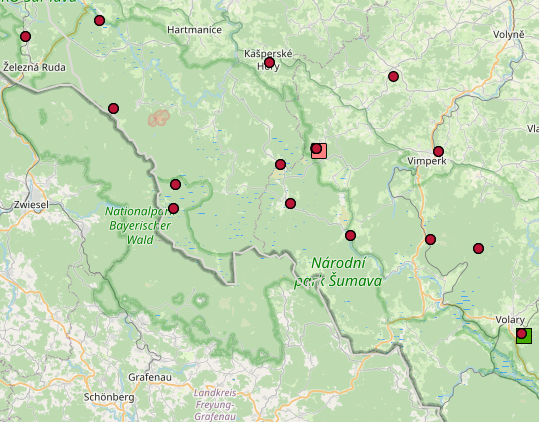
\includegraphics[width=0.6\linewidth]{chmu_stations.png}
		\caption{Mapa Šumavského NP}
	\end{figure}
\end{frame}
%%který stanice mají který veličiny
%------------------------------------------------

\subsection{Data z BÚ AV}

\begin{frame}
	\frametitle{Data z BÚ AV}
	Celkově $\sim$150 čidel.
	\begin{figure}
		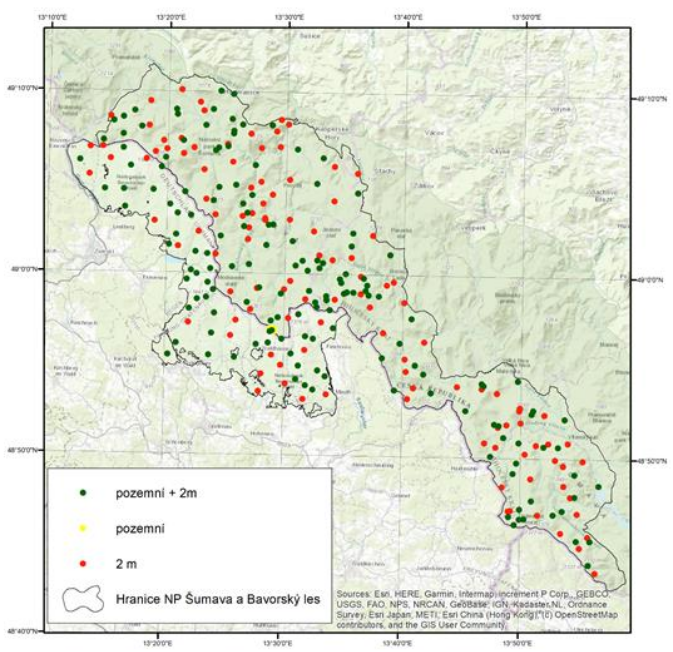
\includegraphics[width=0.7\linewidth]{forest_sensors.png}
		\caption{Rozmístění senzorů}
	\end{figure}
\end{frame}

\begin{frame}
	\frametitle{Data from BÚ AV}
	\begin{figure}
		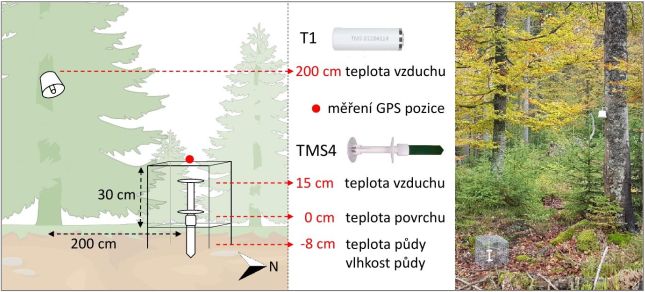
\includegraphics[width=0.8\linewidth]{sensor_closeup.png}
		\caption{Poloha senzoru}
	\end{figure}
\end{frame}



%------------------------------------------------

\section{Metody a výsledky}

\subsection{Metody}

\begin{frame}
	\begin{itemize}
		\item Z dat ČHMÚ máme prediktory: výška sněhu, oblačnost, 10 minutové srážky, rychlost větru
	
\item K tomu: měsíc v roce, vhlkost

\item Použijeme mnohonásobnou lineární regresi pro každé čidlo (minimální, maximální teplota)
	\end{itemize}
\end{frame}

\begin{frame}
	\begin{figure}
		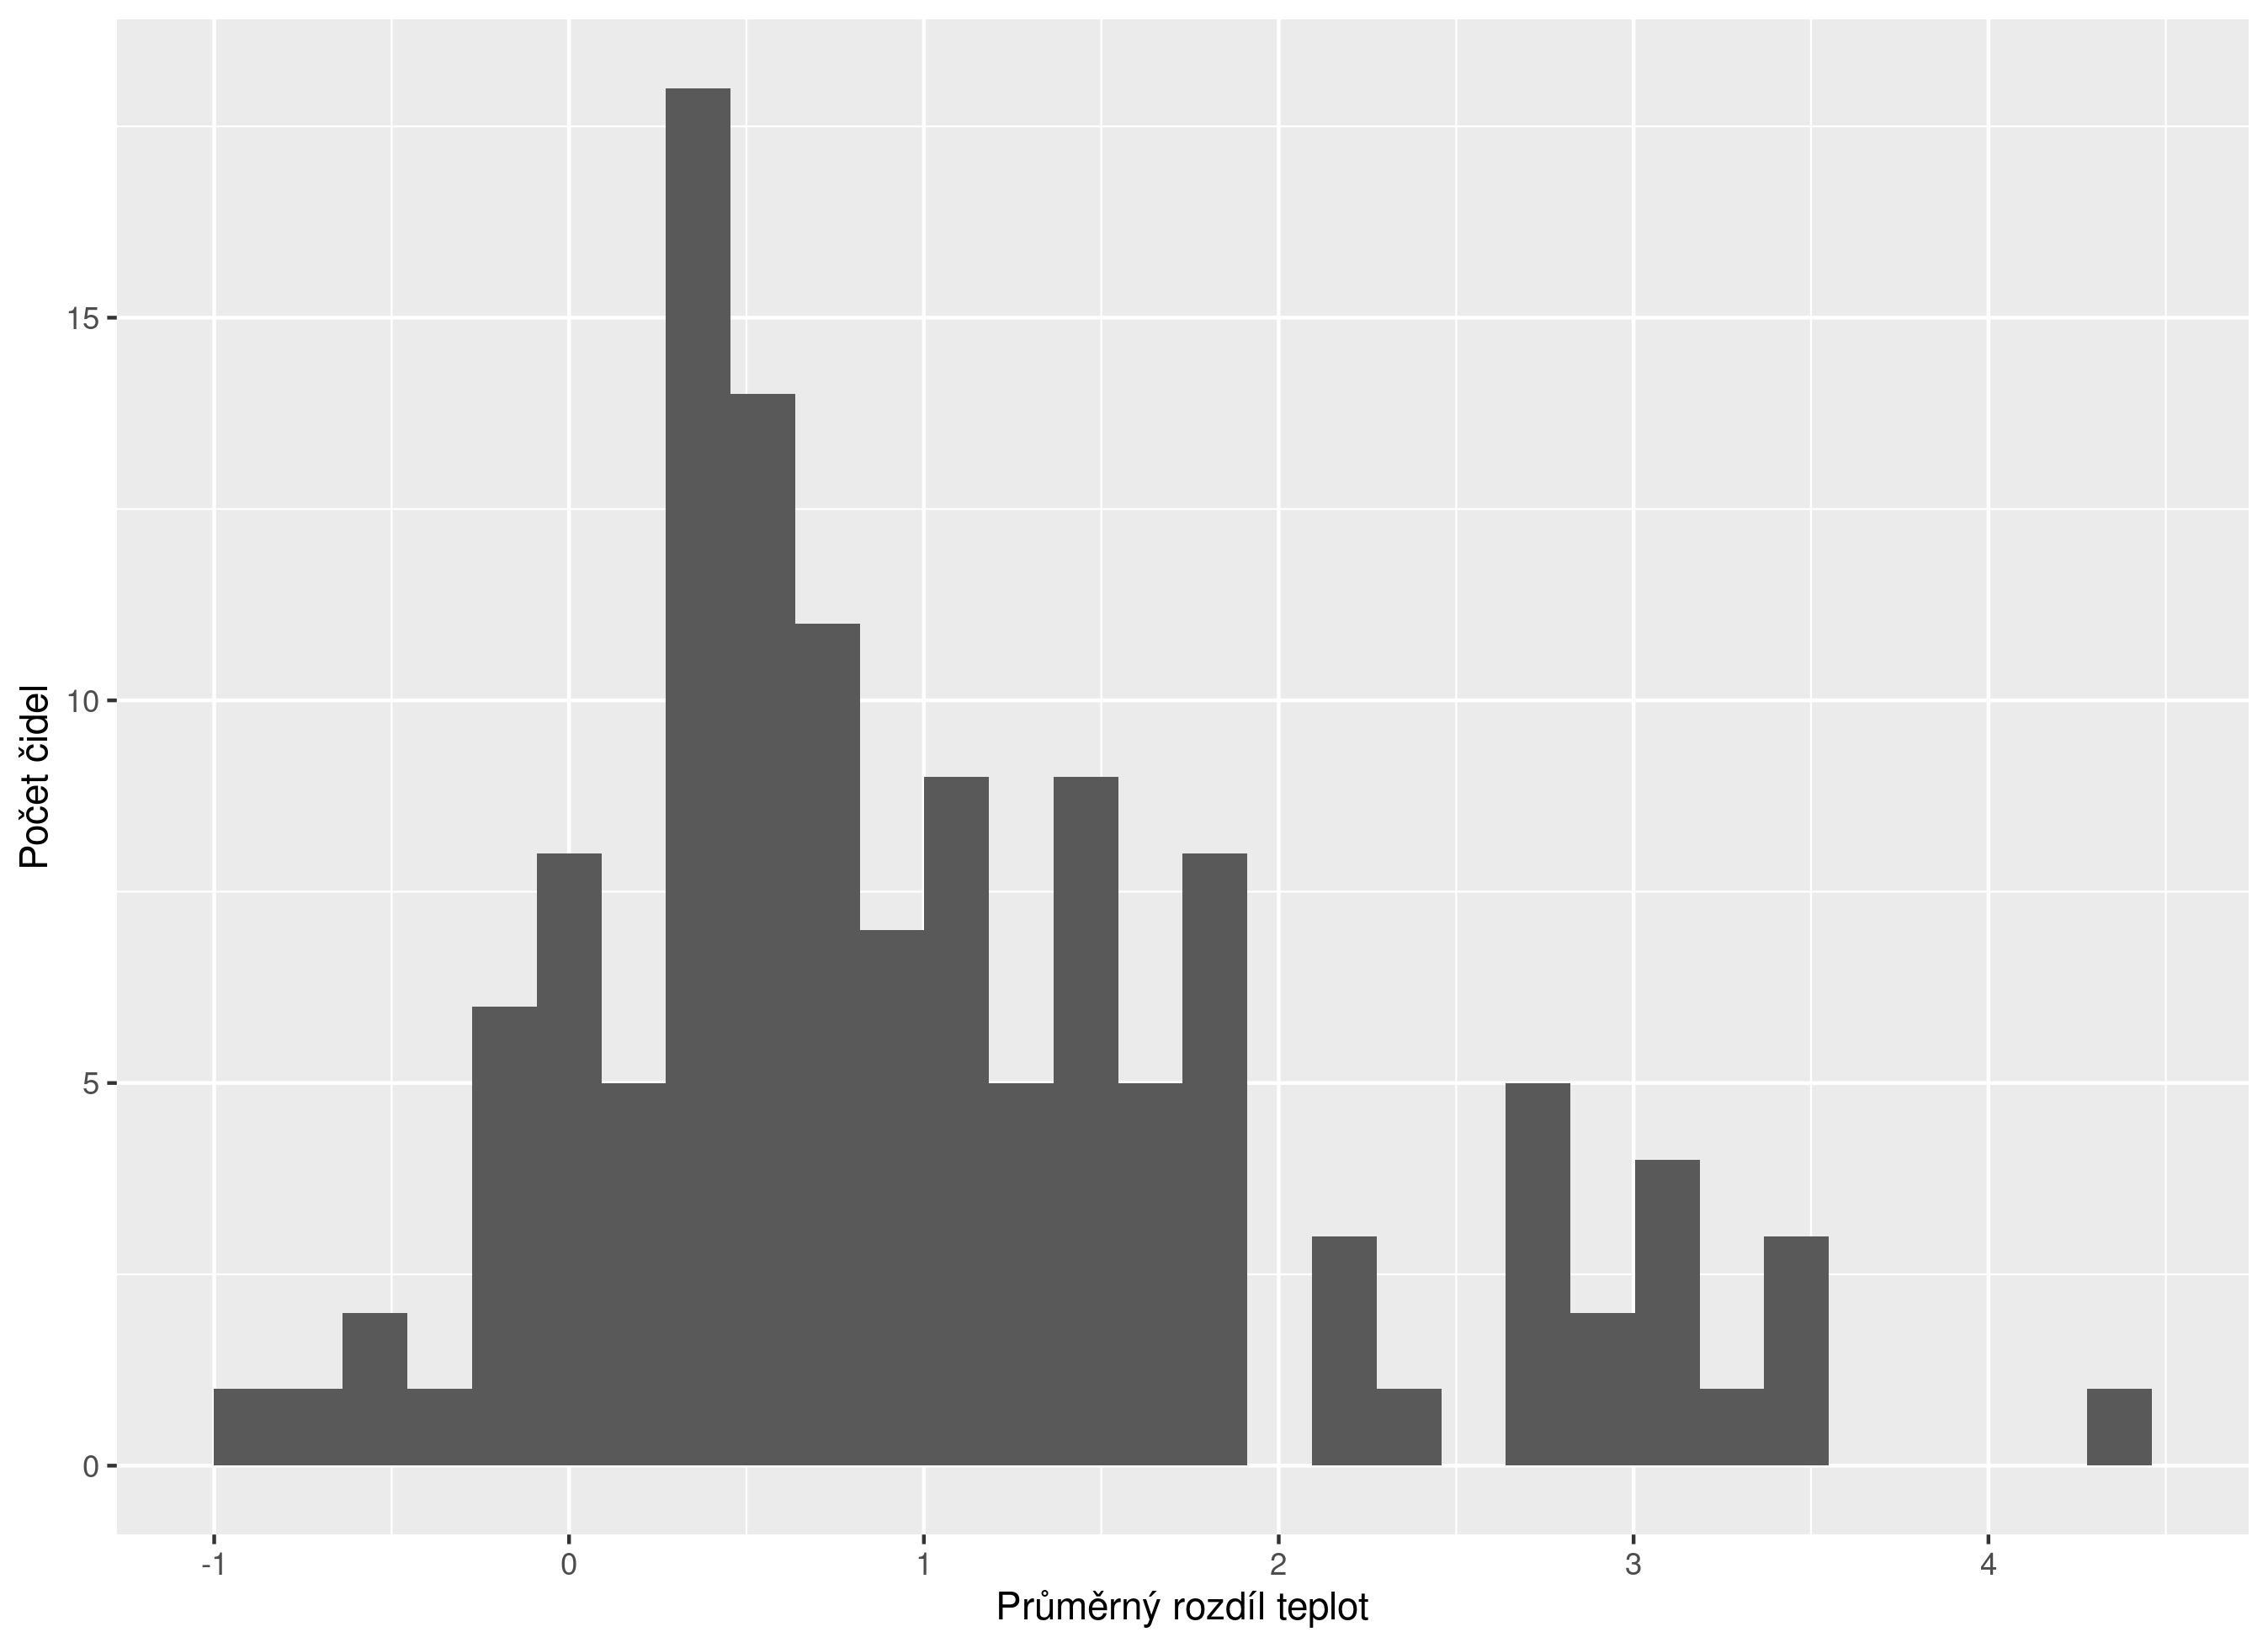
\includegraphics[width=0.8\linewidth,height=0.6\textwidth]{hist.png}
		\caption{Histogram průměrného rozdílu maximálních teplot mezi $\SI{15}{cm}$ a $\SI{2}{m}$}
	\end{figure}
\end{frame}

\begin{frame}
	\begin{figure}
		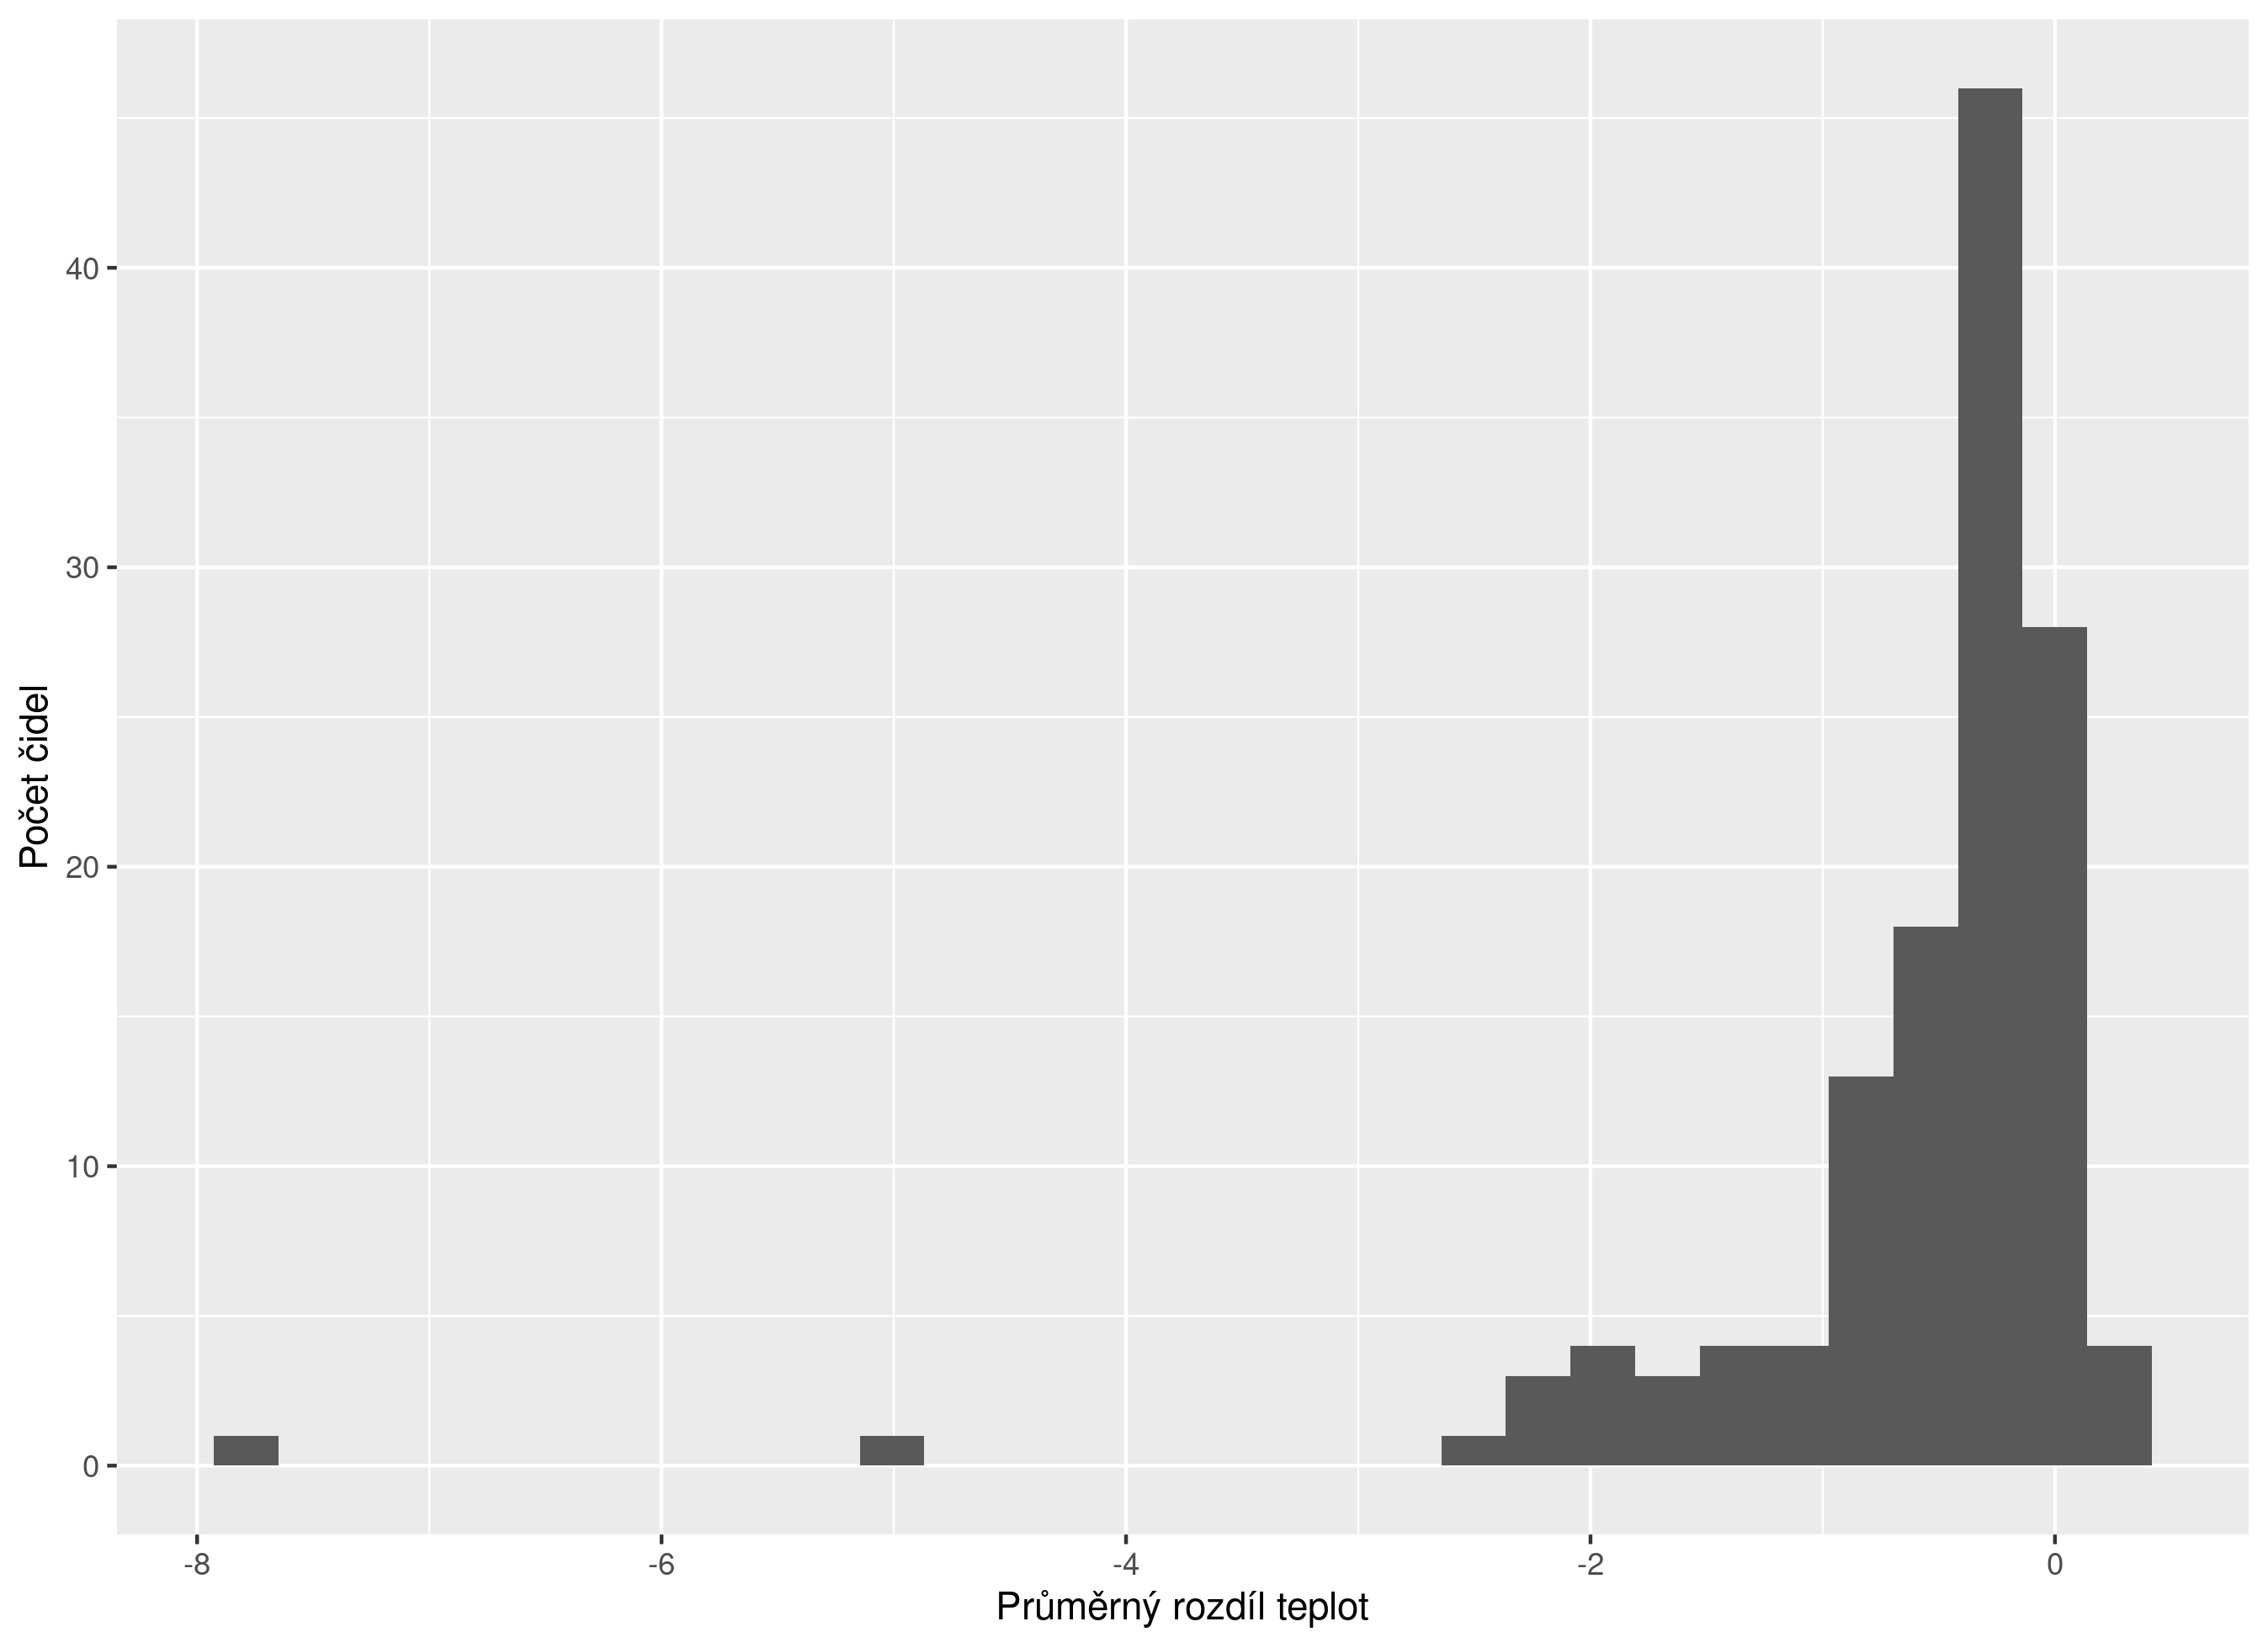
\includegraphics[width=0.8\linewidth,height=0.6\textwidth]{hist2.png}
		\caption{Histogram průměrného rozdílu minimálních teplot mezi $\SI{15}{cm}$ a $\SI{2}{m}$}
	\end{figure}
\end{frame}
%------------------------------------------------

\subsection{Výsledky}

\begin{frame}
	\frametitle{Závislost na vzdálenosti}
	\begin{figure}
		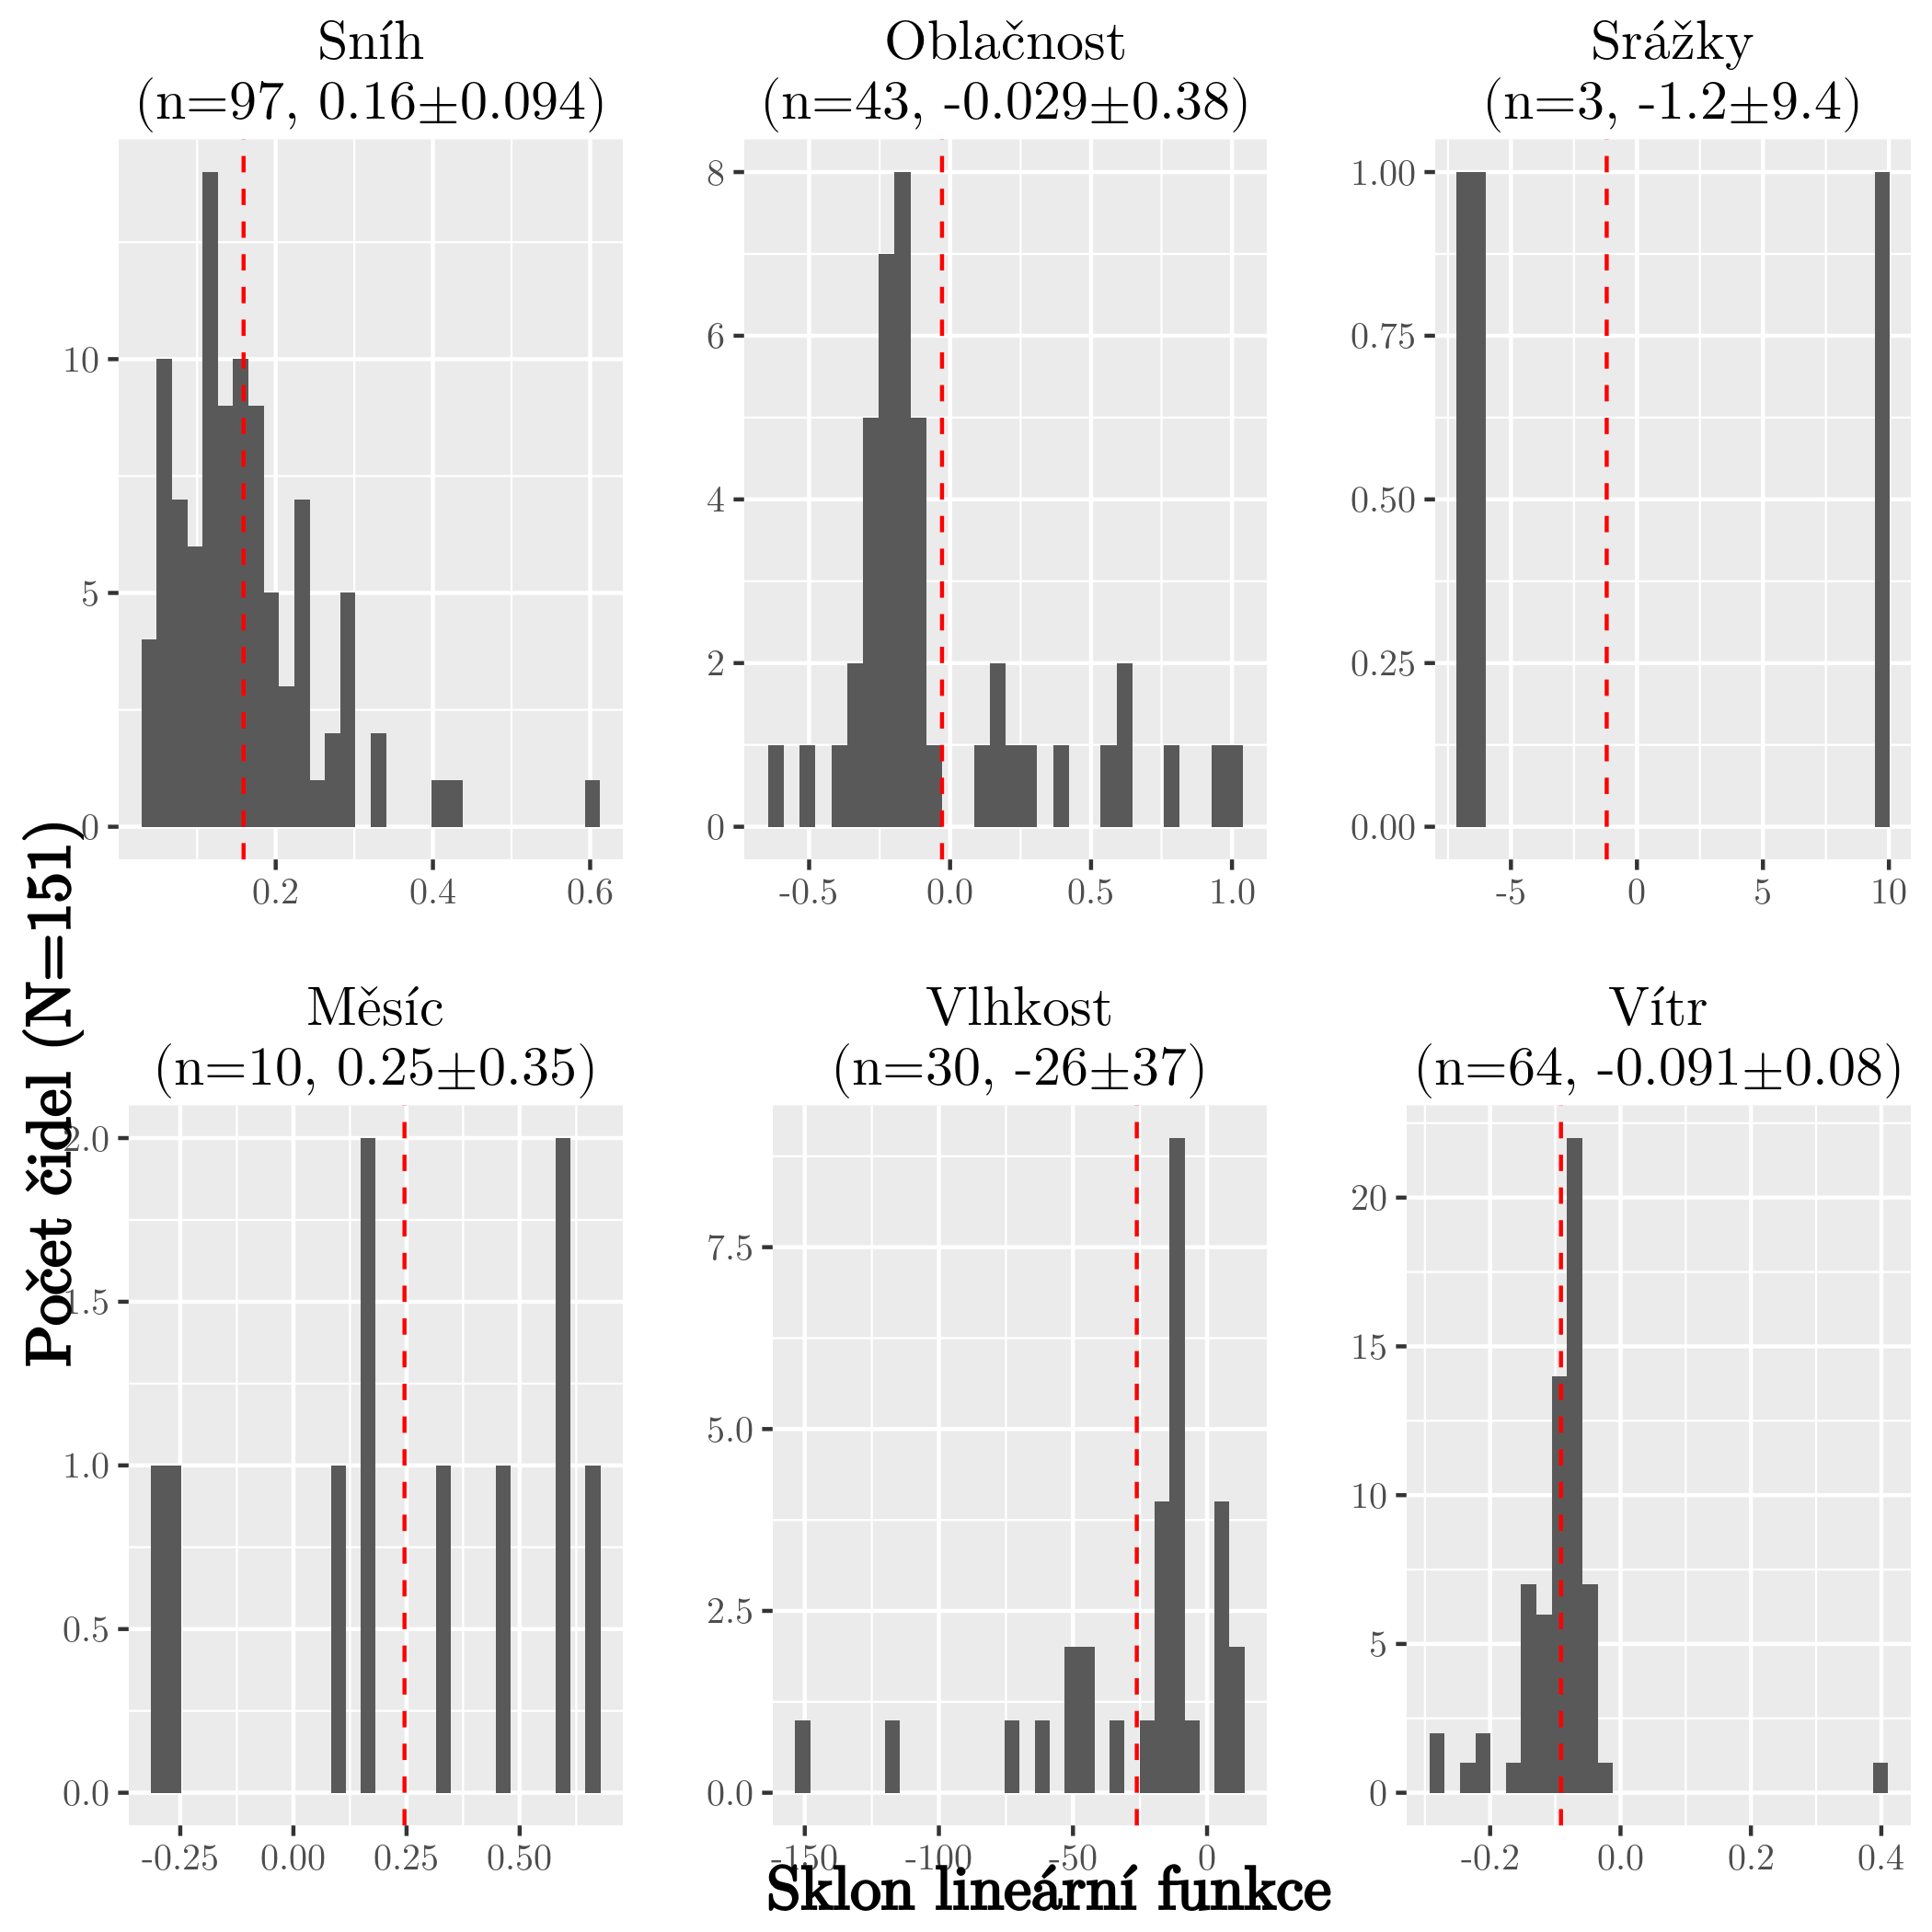
\includegraphics[width=0.8\linewidth,height=0.6\textwidth]{all151minTall0cm_BWyes.png}
		\caption{Všechna čidla, minimální denní teplota v $\SI{0}{cm}$}
	\end{figure}
\end{frame}

\begin{frame}
	\frametitle{Závislost na vzdálenosti}
	\begin{figure}
		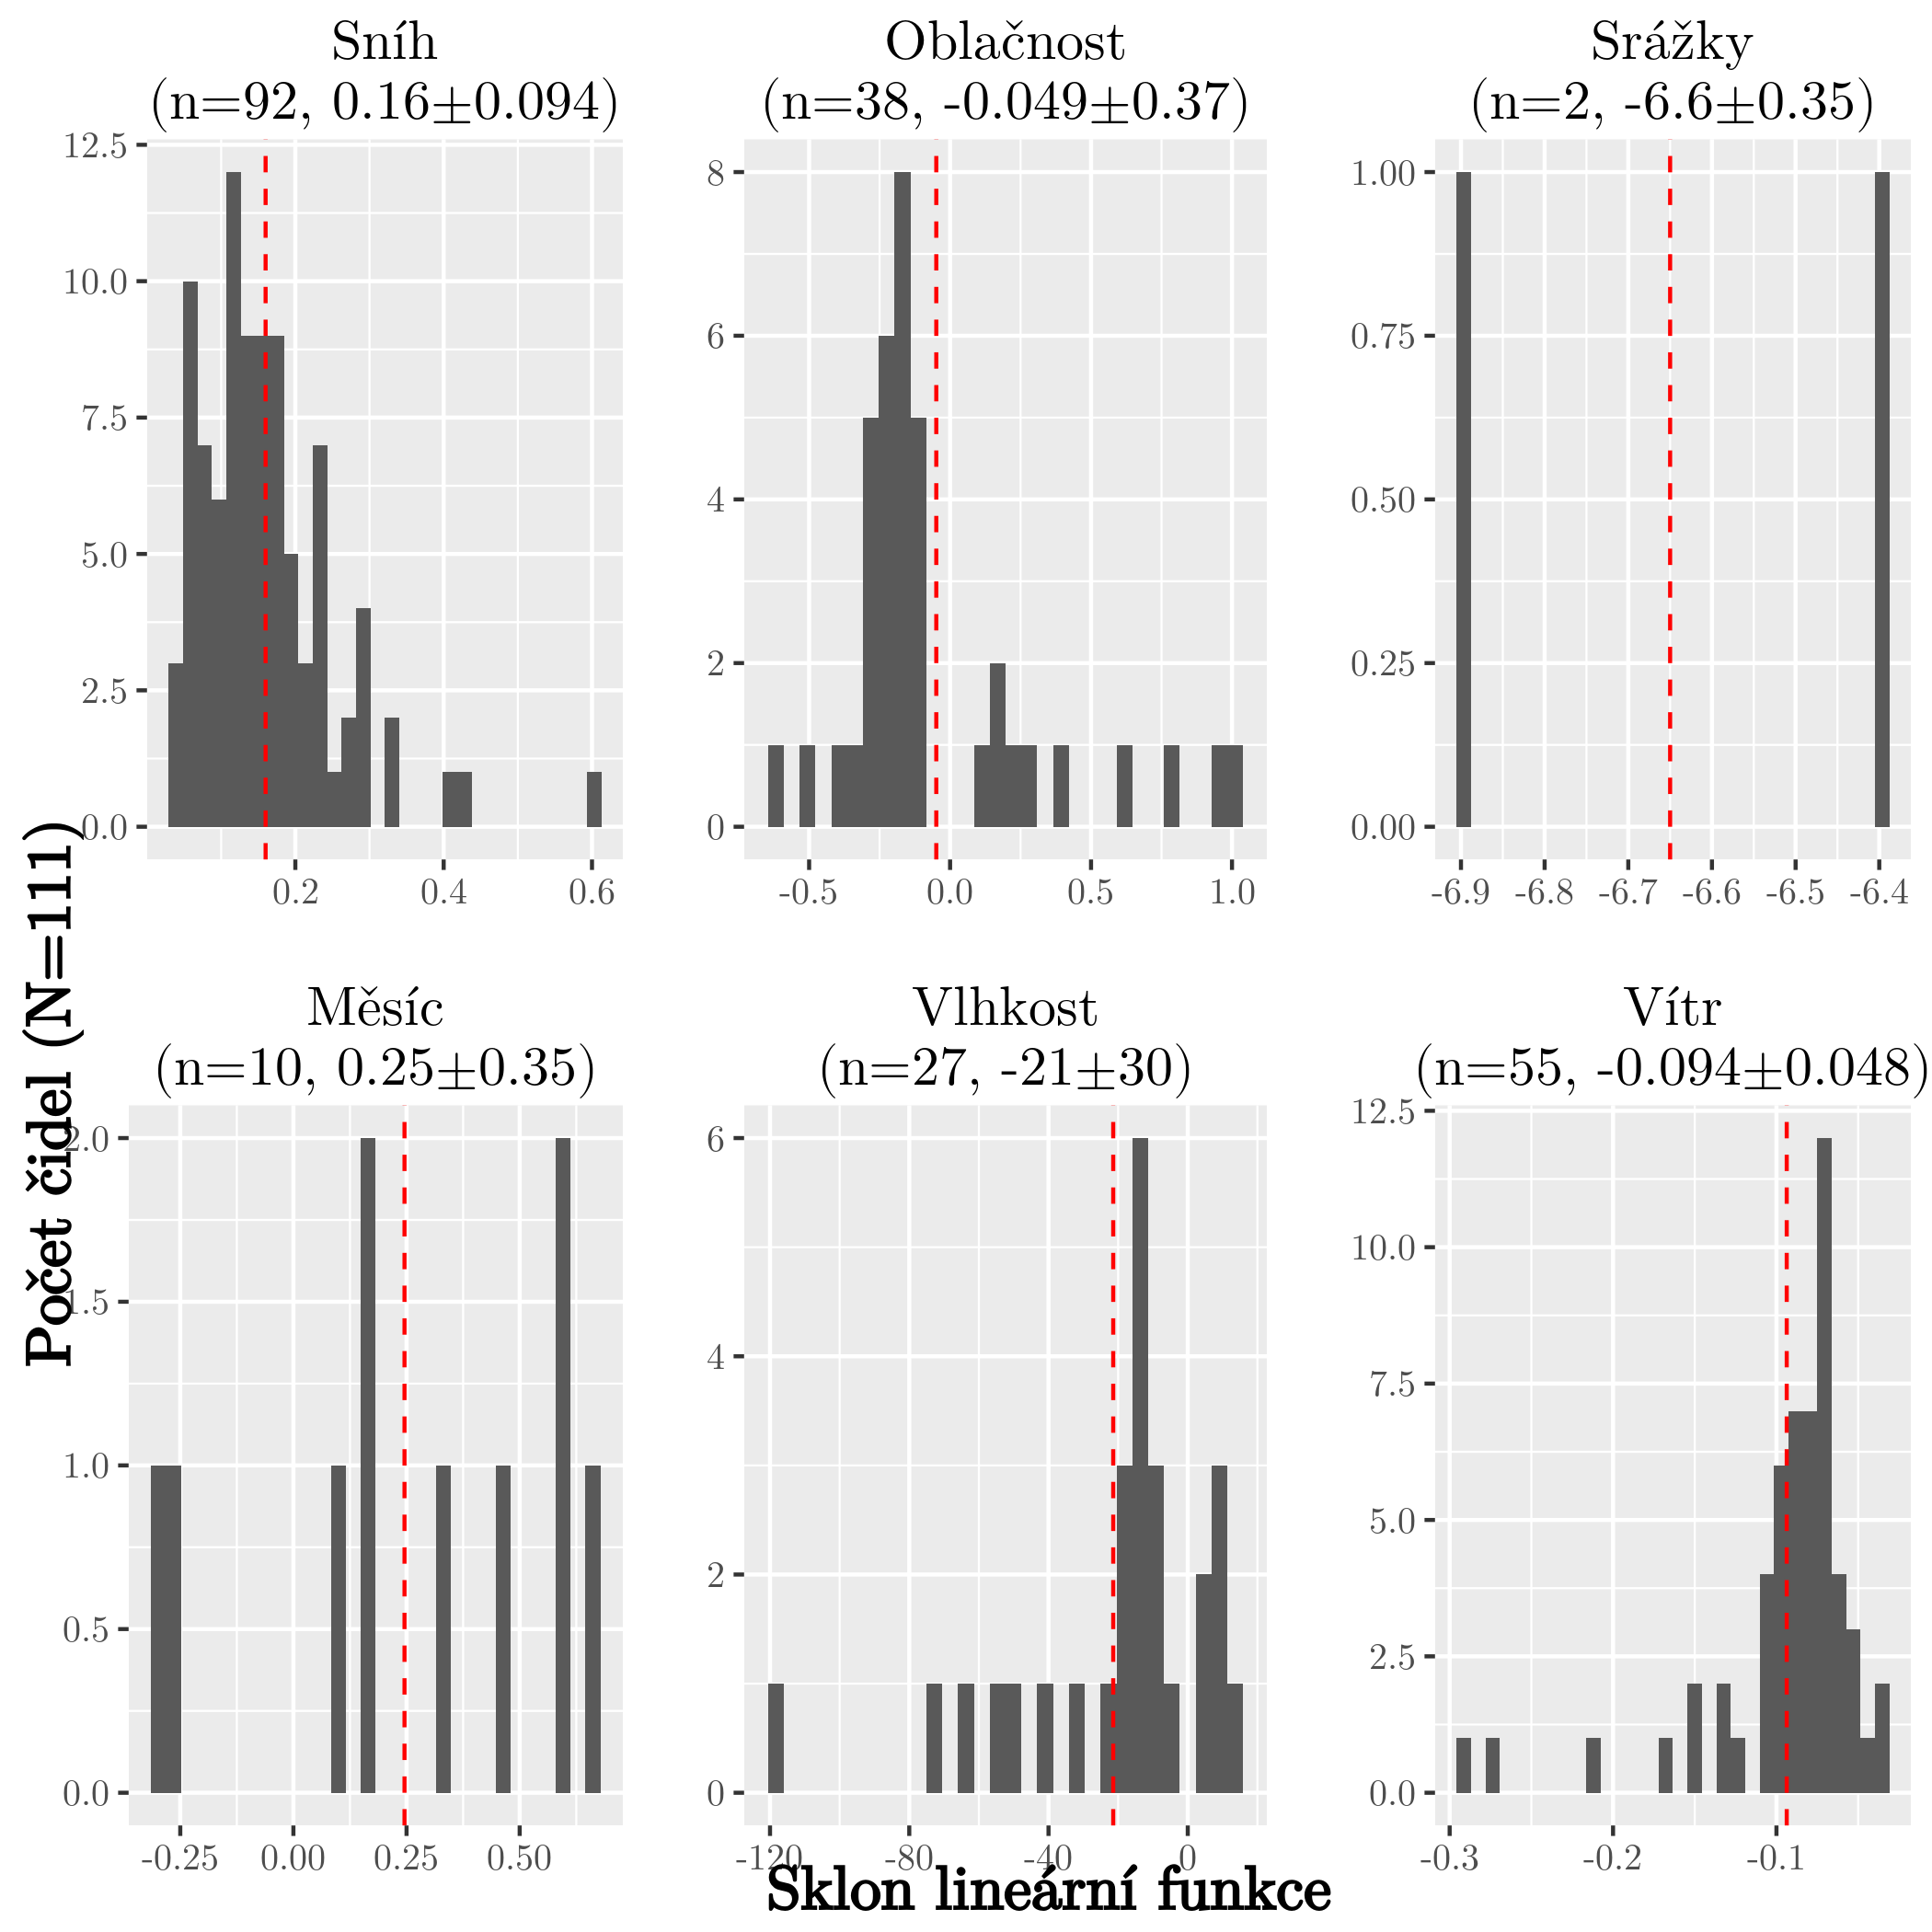
\includegraphics[width=0.8\linewidth,height=0.6\textwidth]{all111minTall0cm_BWno.png}
		\caption{Čidla v NP Šumava, minimální denní teplota v $\SI{0}{cm}$}
	\end{figure}
\end{frame}

\begin{frame}
	\frametitle{Závislost na vzdálenosti}
	\begin{figure}
		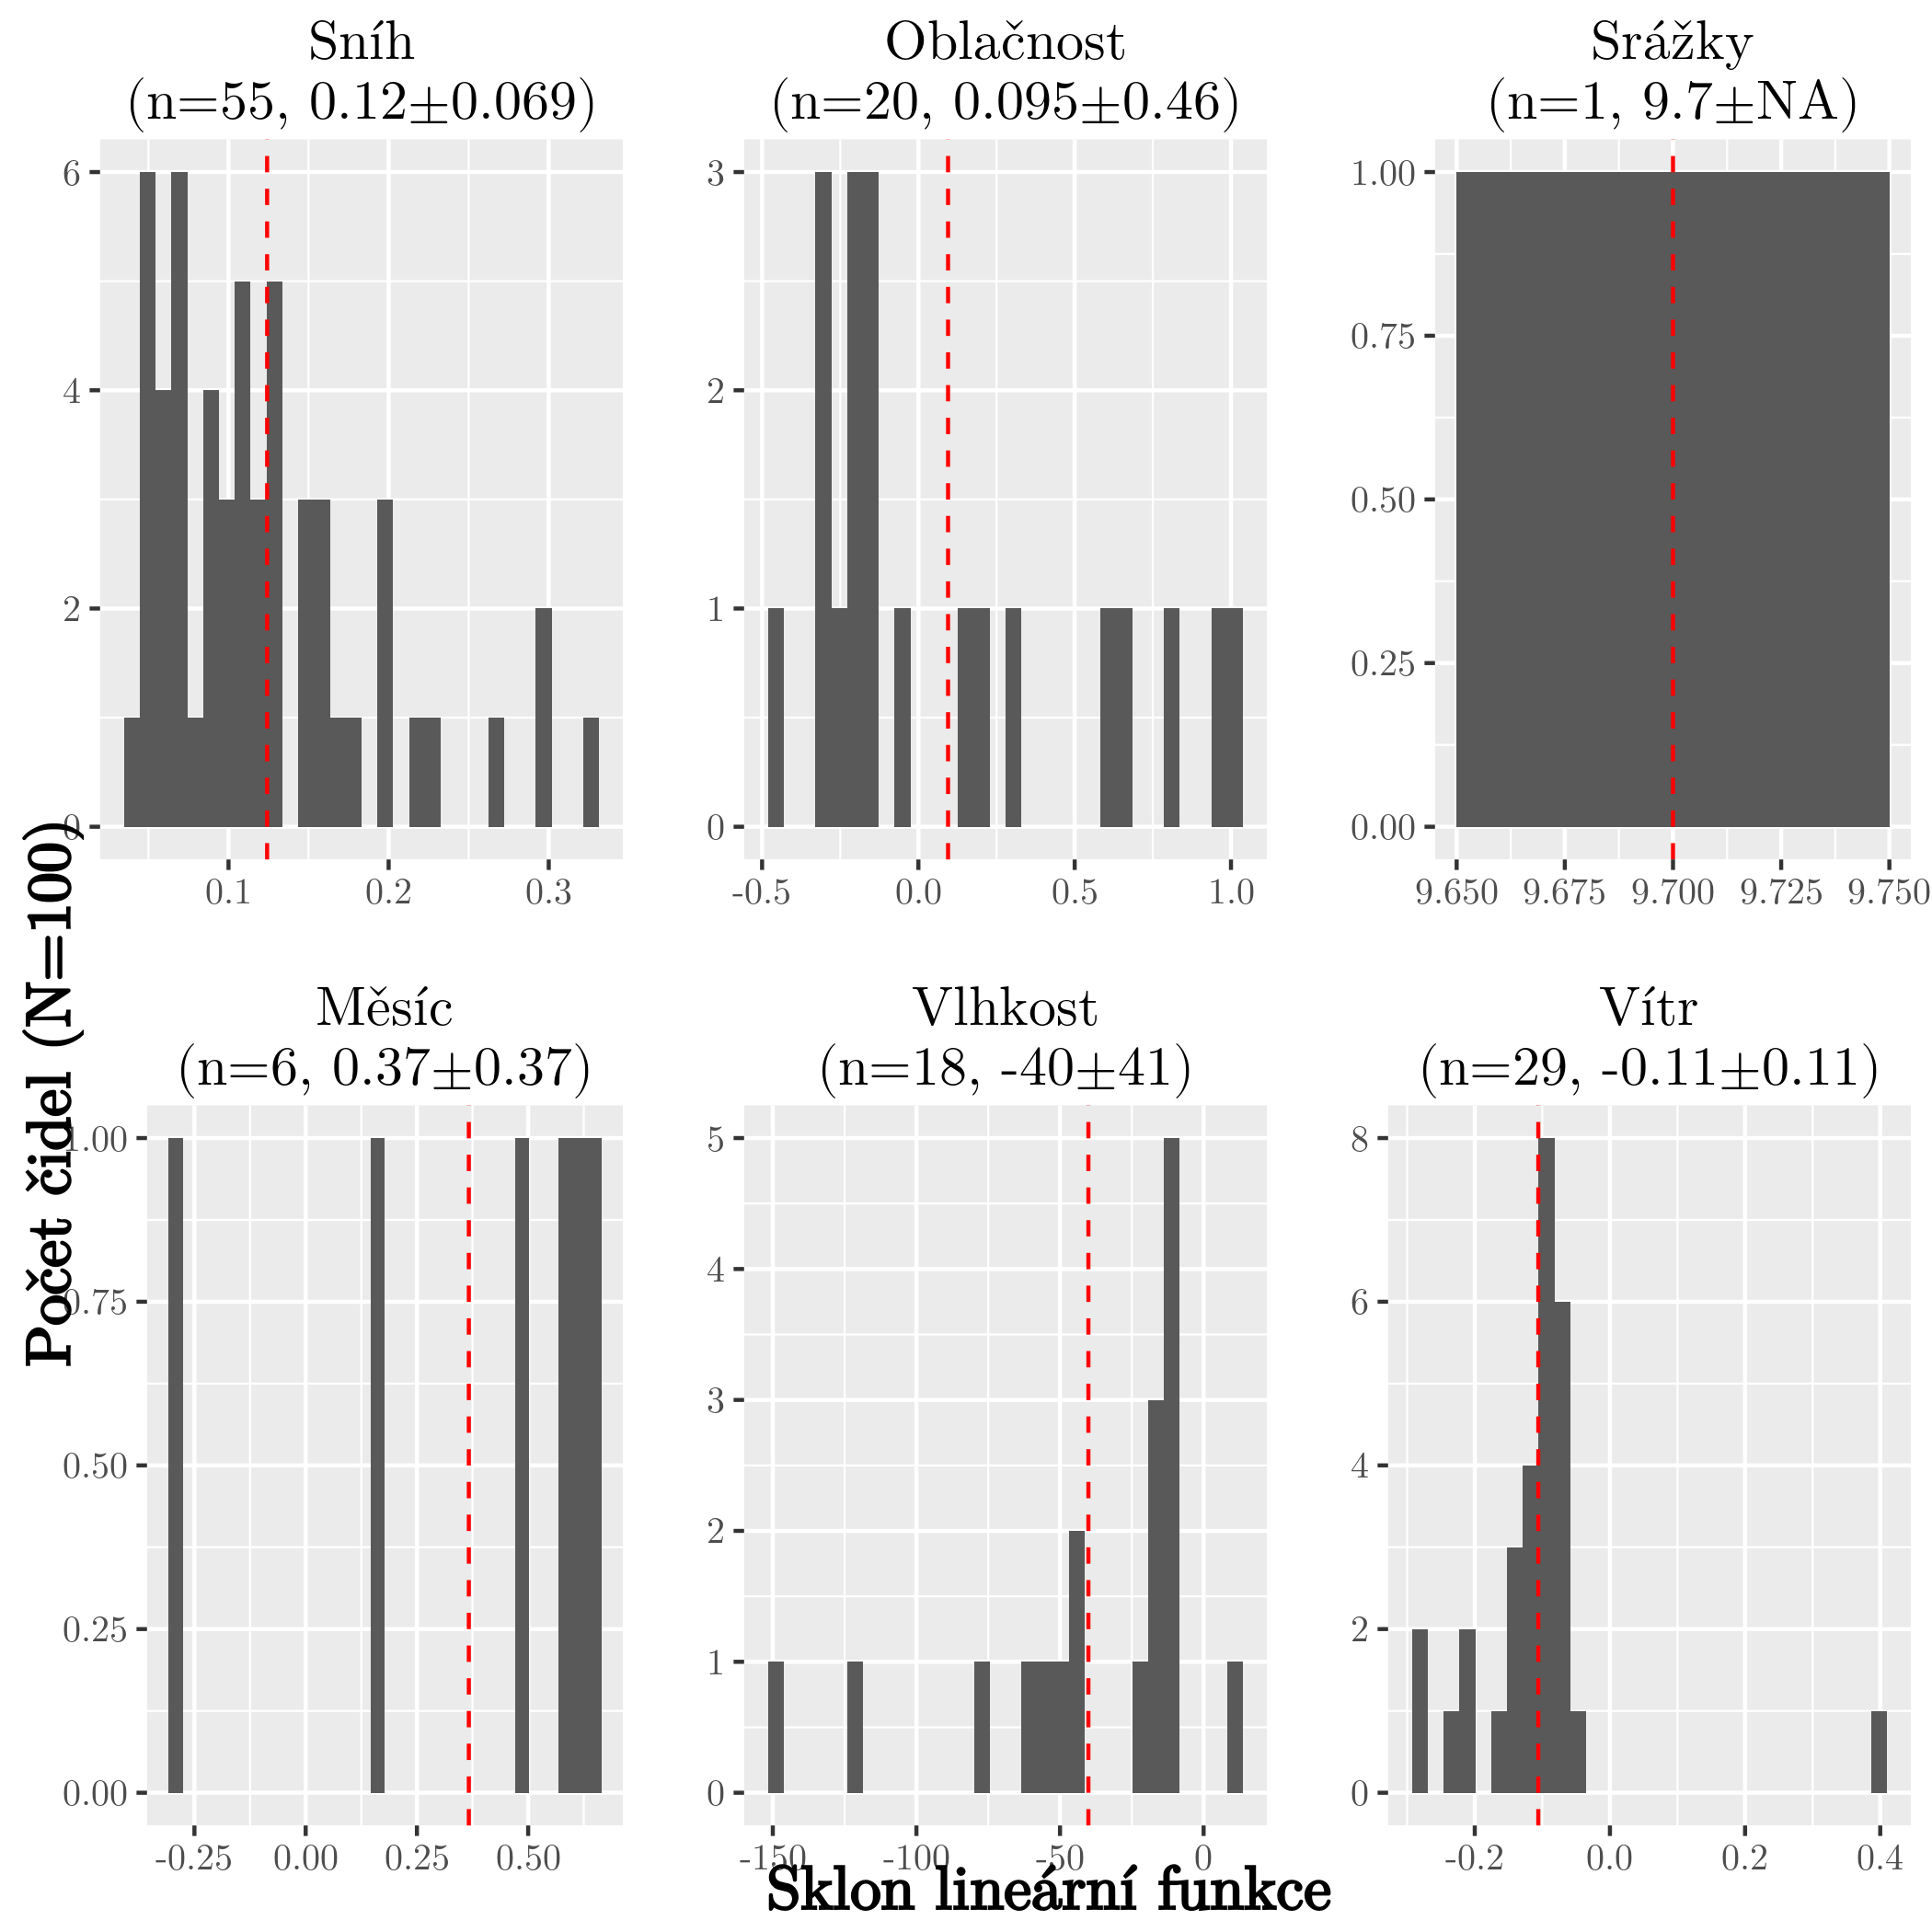
\includegraphics[width=0.8\linewidth,height=0.6\textwidth]{all100minTall0cm_BWyesc4japi0120000.png}
		\caption{Čidla ve vzdálenosti $\SI{20}{km}$ od Javoří Pily, minimální denní teplota v $\SI{0}{cm}$}
	\end{figure}
\end{frame}

\begin{frame}
	\frametitle{Závislost na vzdálenosti}
	\begin{figure}
		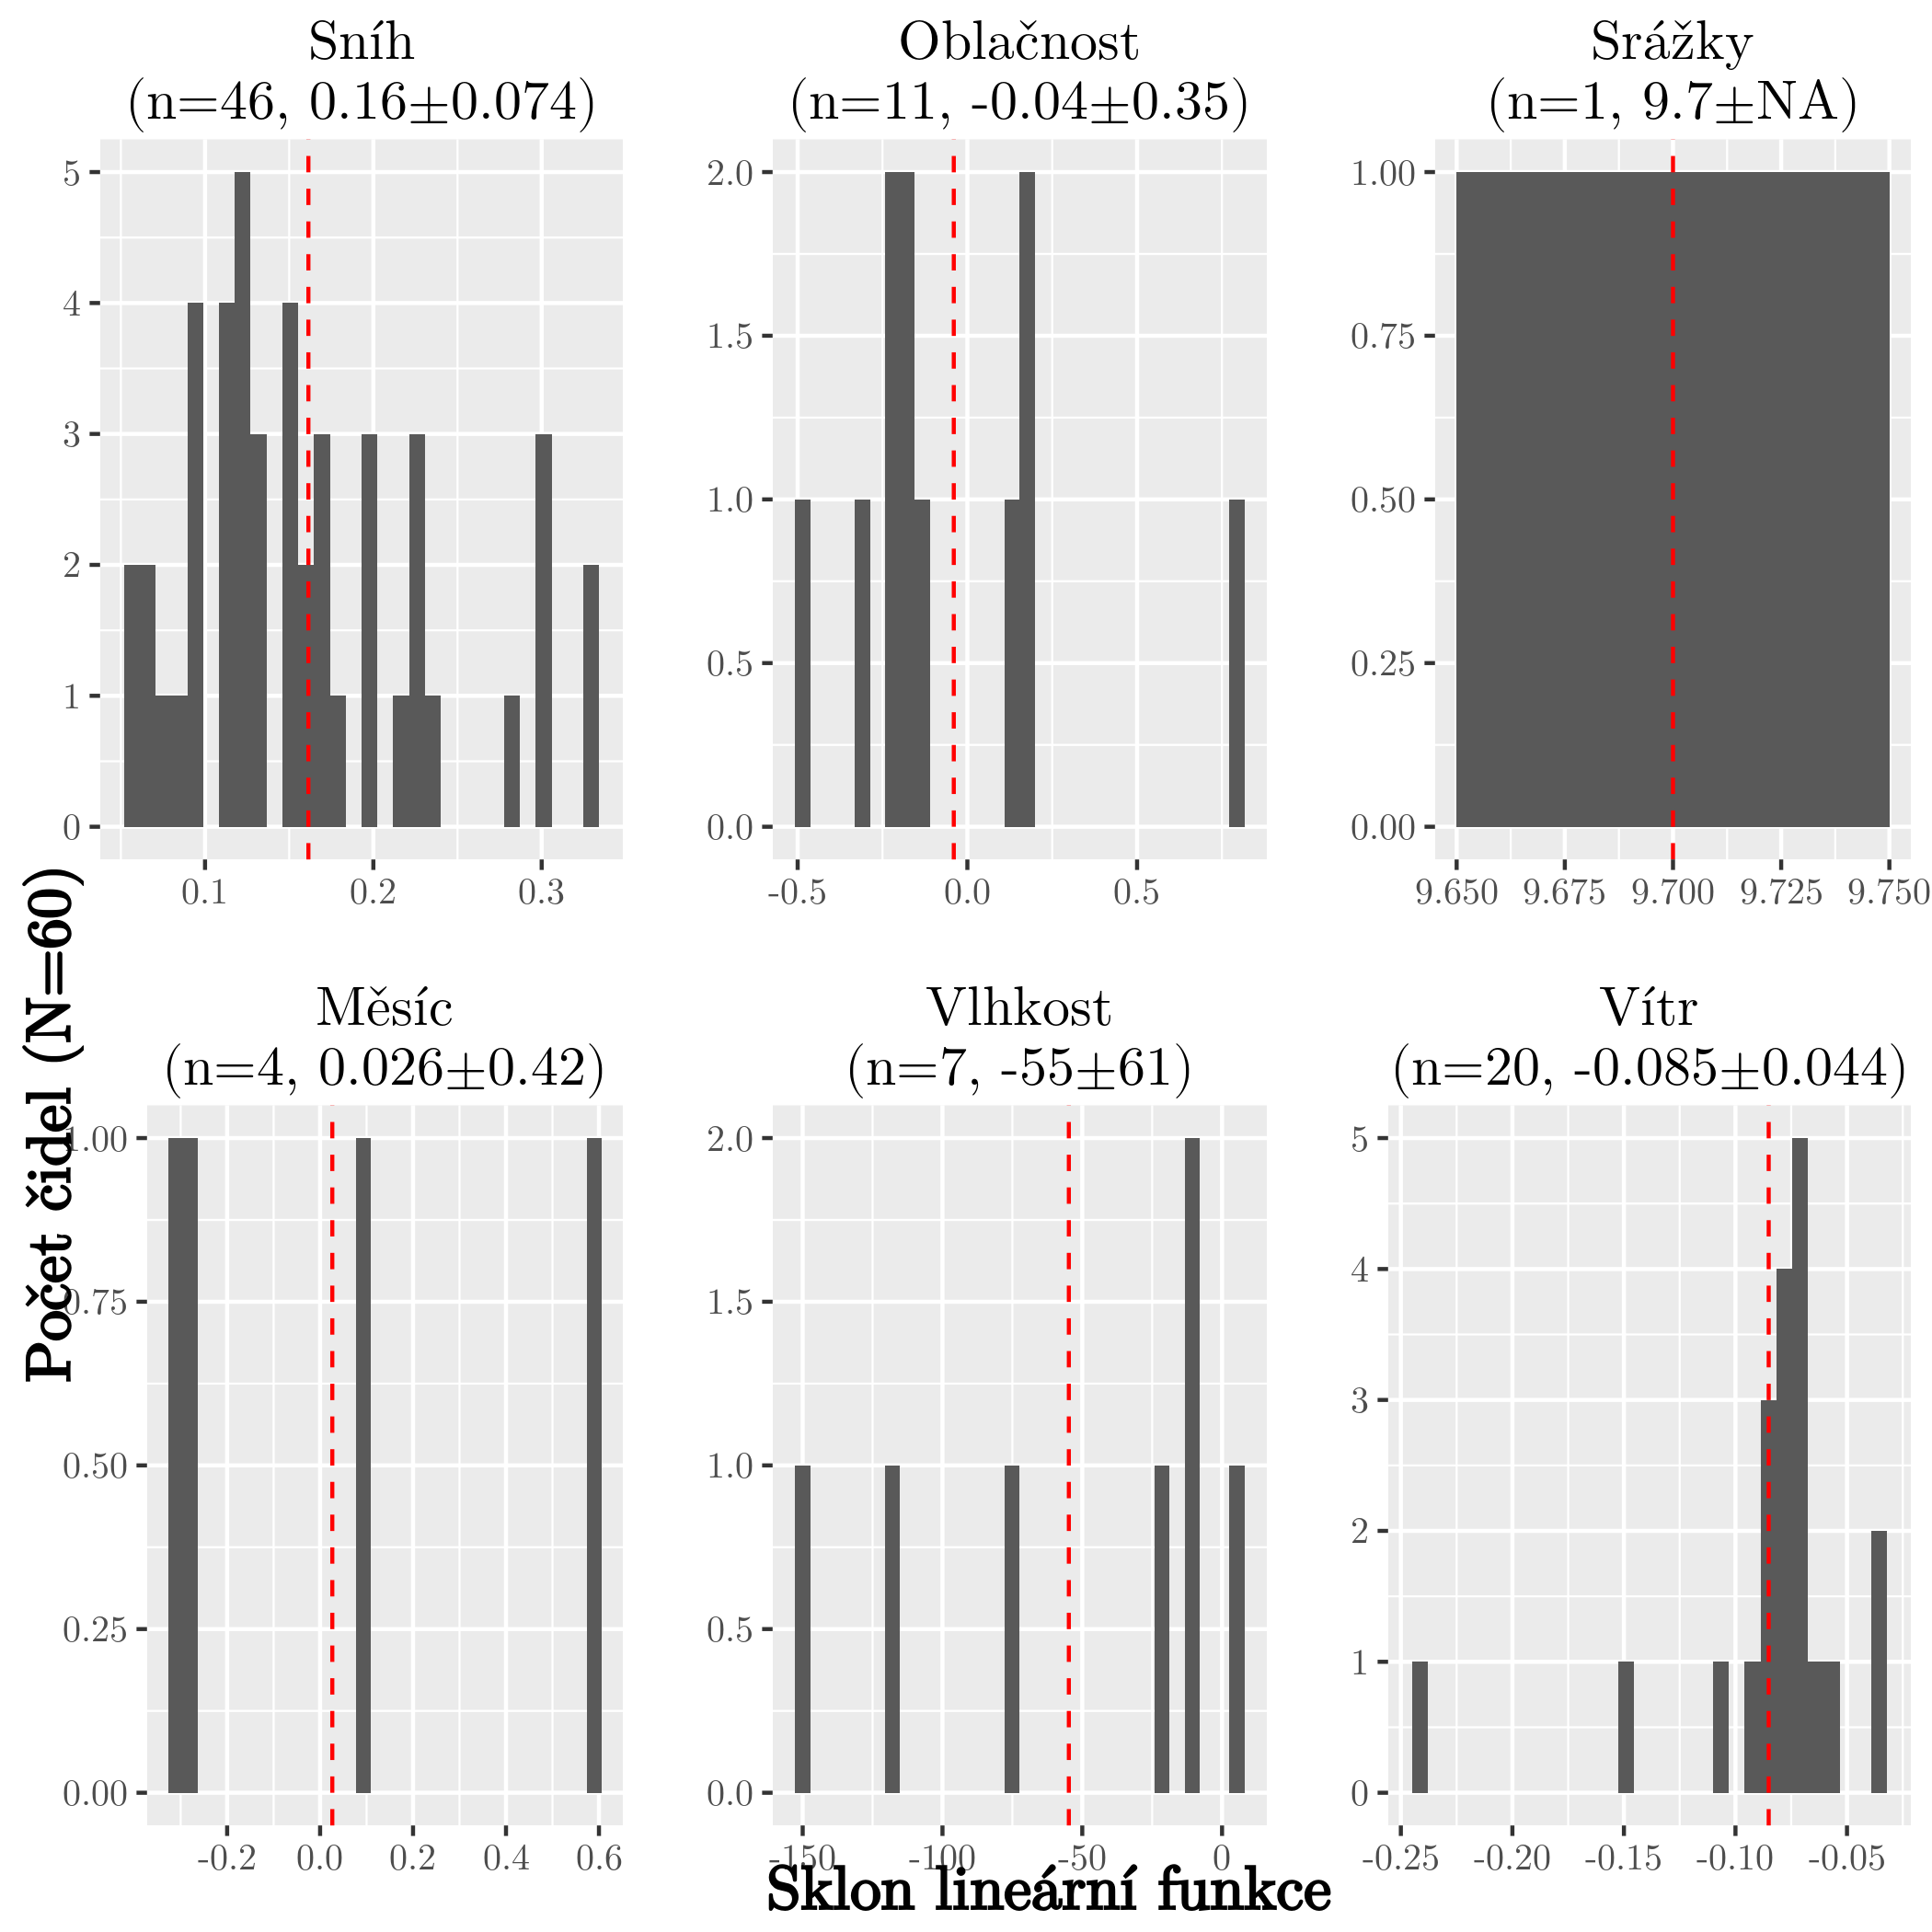
\includegraphics[width=0.8\linewidth,height=0.6\textwidth]{all60minTall0cm_BWyesc1chur0120000.png}
		\caption{Čidla ve vzdálenosti $\SI{20}{km}$ od Churáňova, minimální denní teplota v $\SI{0}{cm}$}
	\end{figure}
\end{frame}

\begin{frame}
	\frametitle{Maximální teploty}
	\begin{figure}
		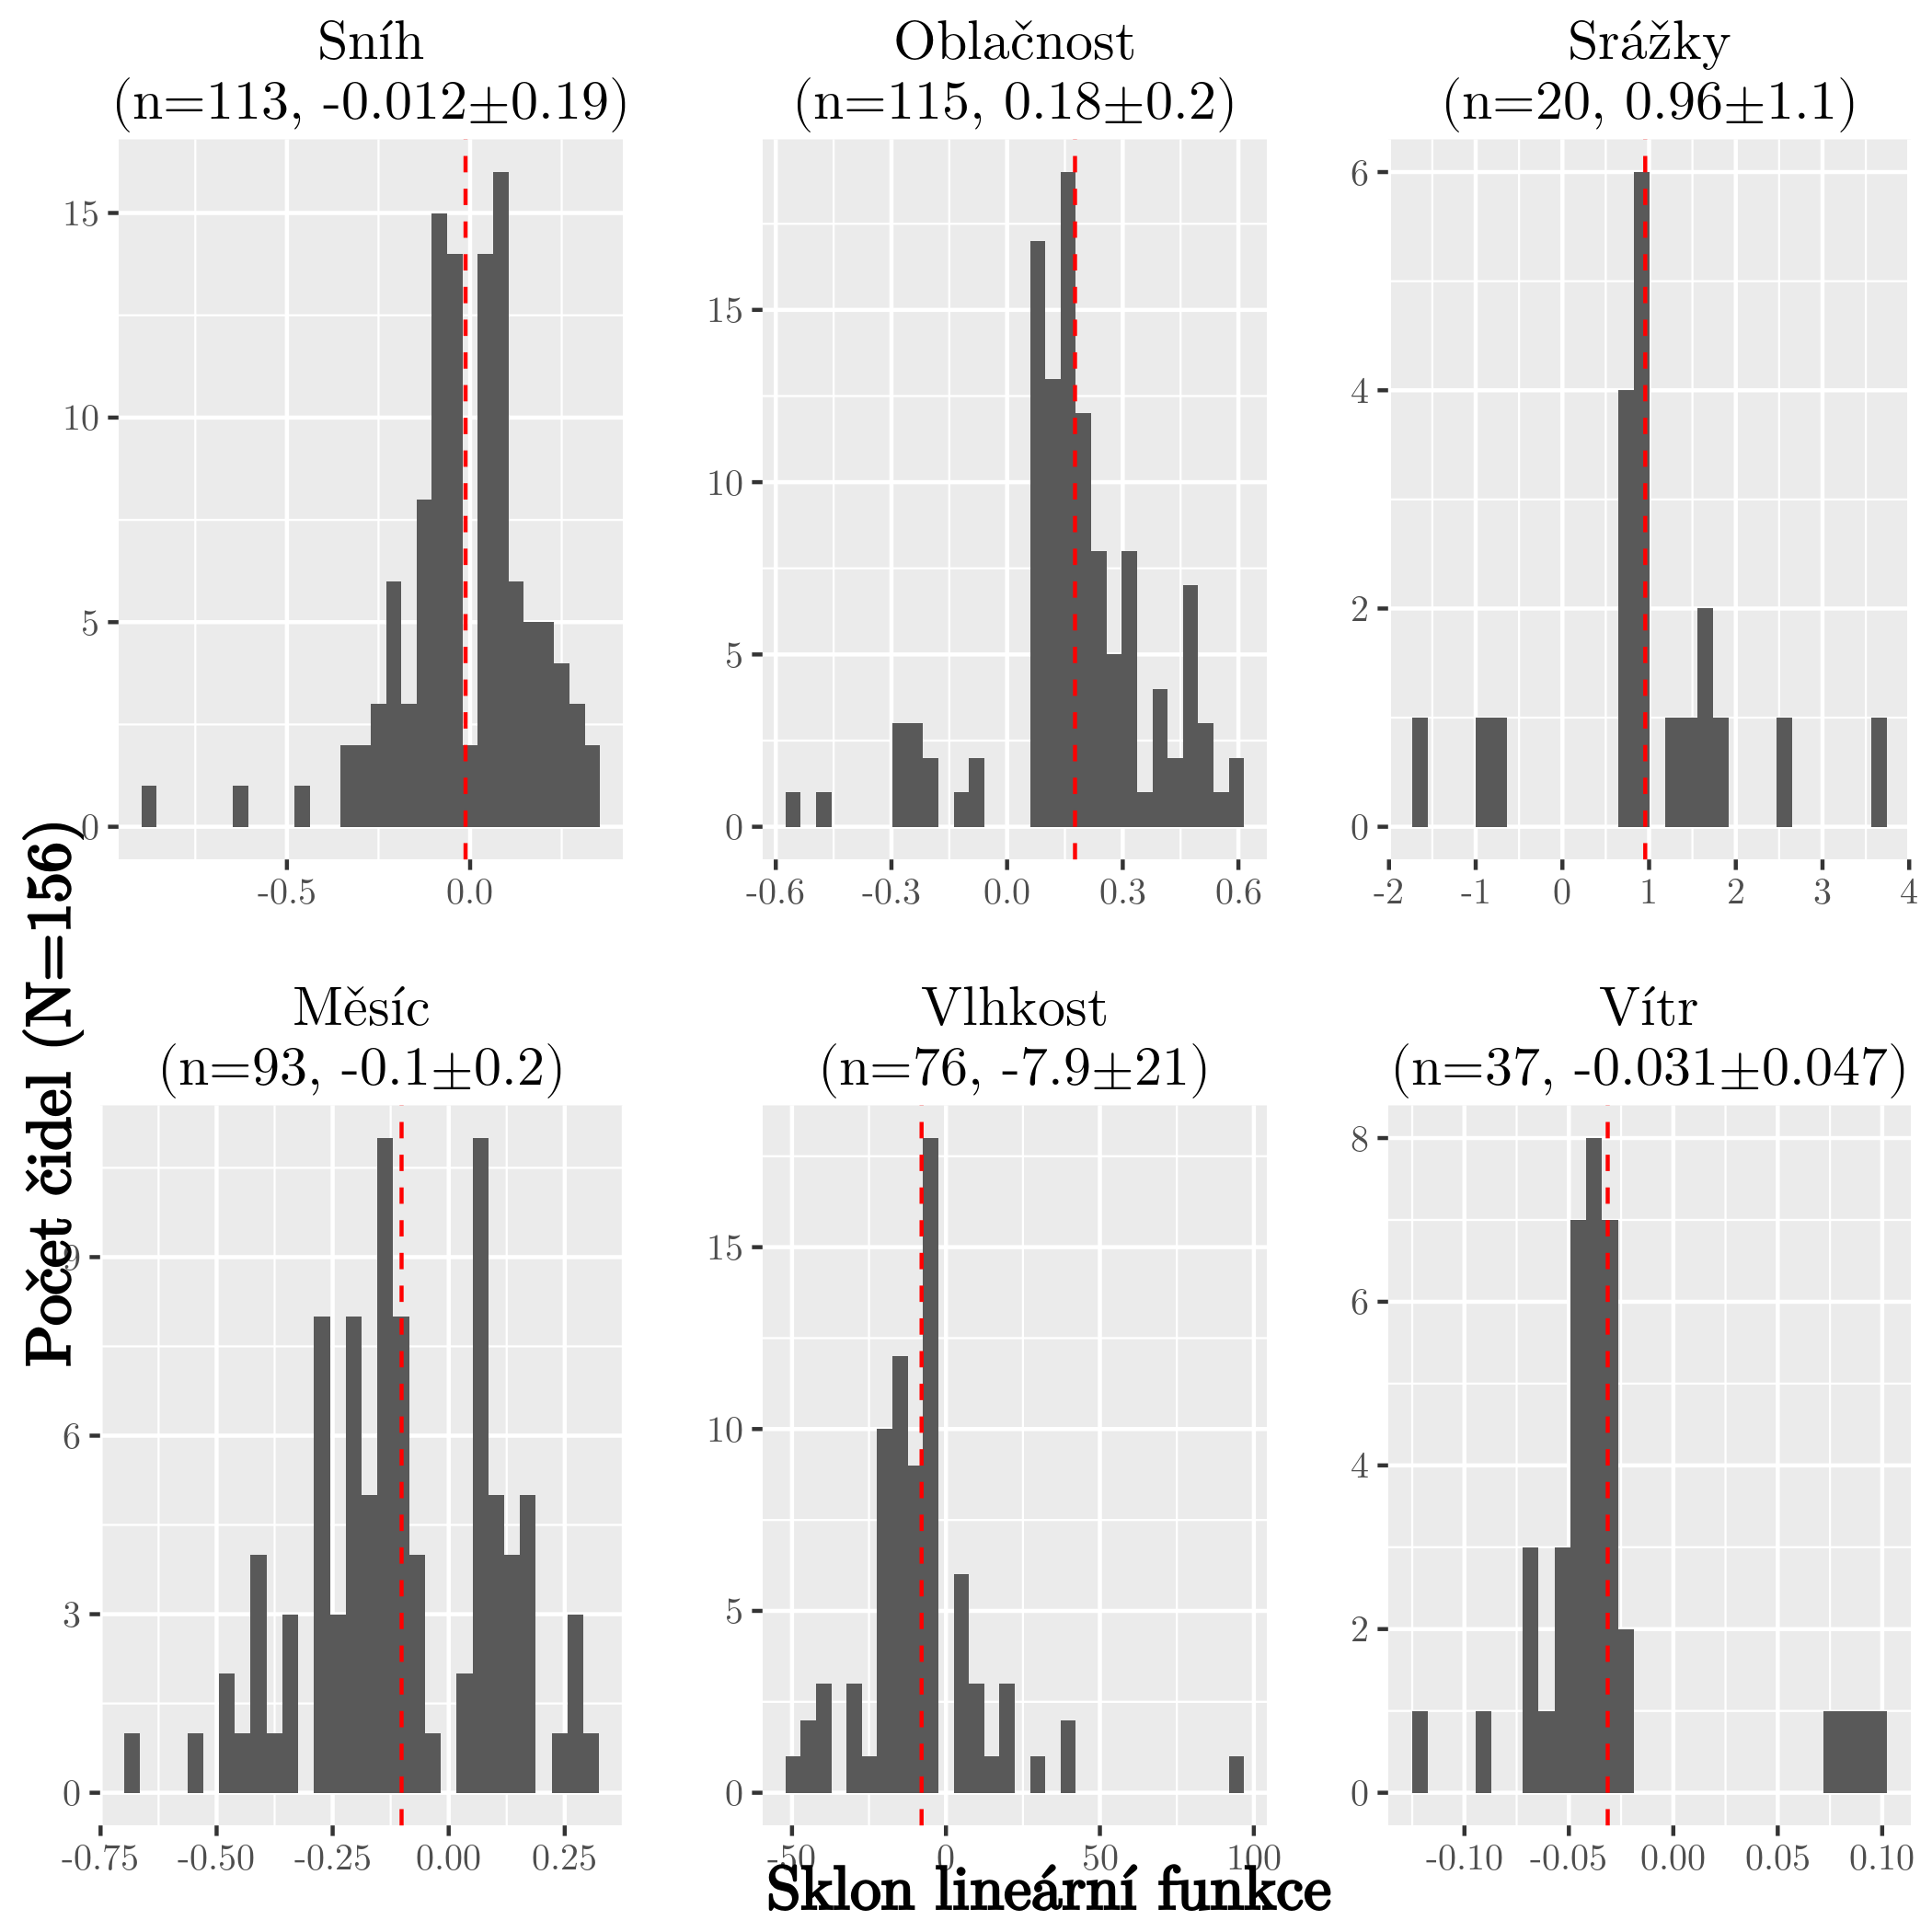
\includegraphics[width=0.8\linewidth,height=0.6\textwidth]{all156maxTall0cm_BWyes.png}
		\caption{Maximální denní teplota v $\SI{0}{cm}$}
	\end{figure}
\end{frame}

\begin{frame}
	\frametitle{Maximální teploty}
	\begin{figure}
		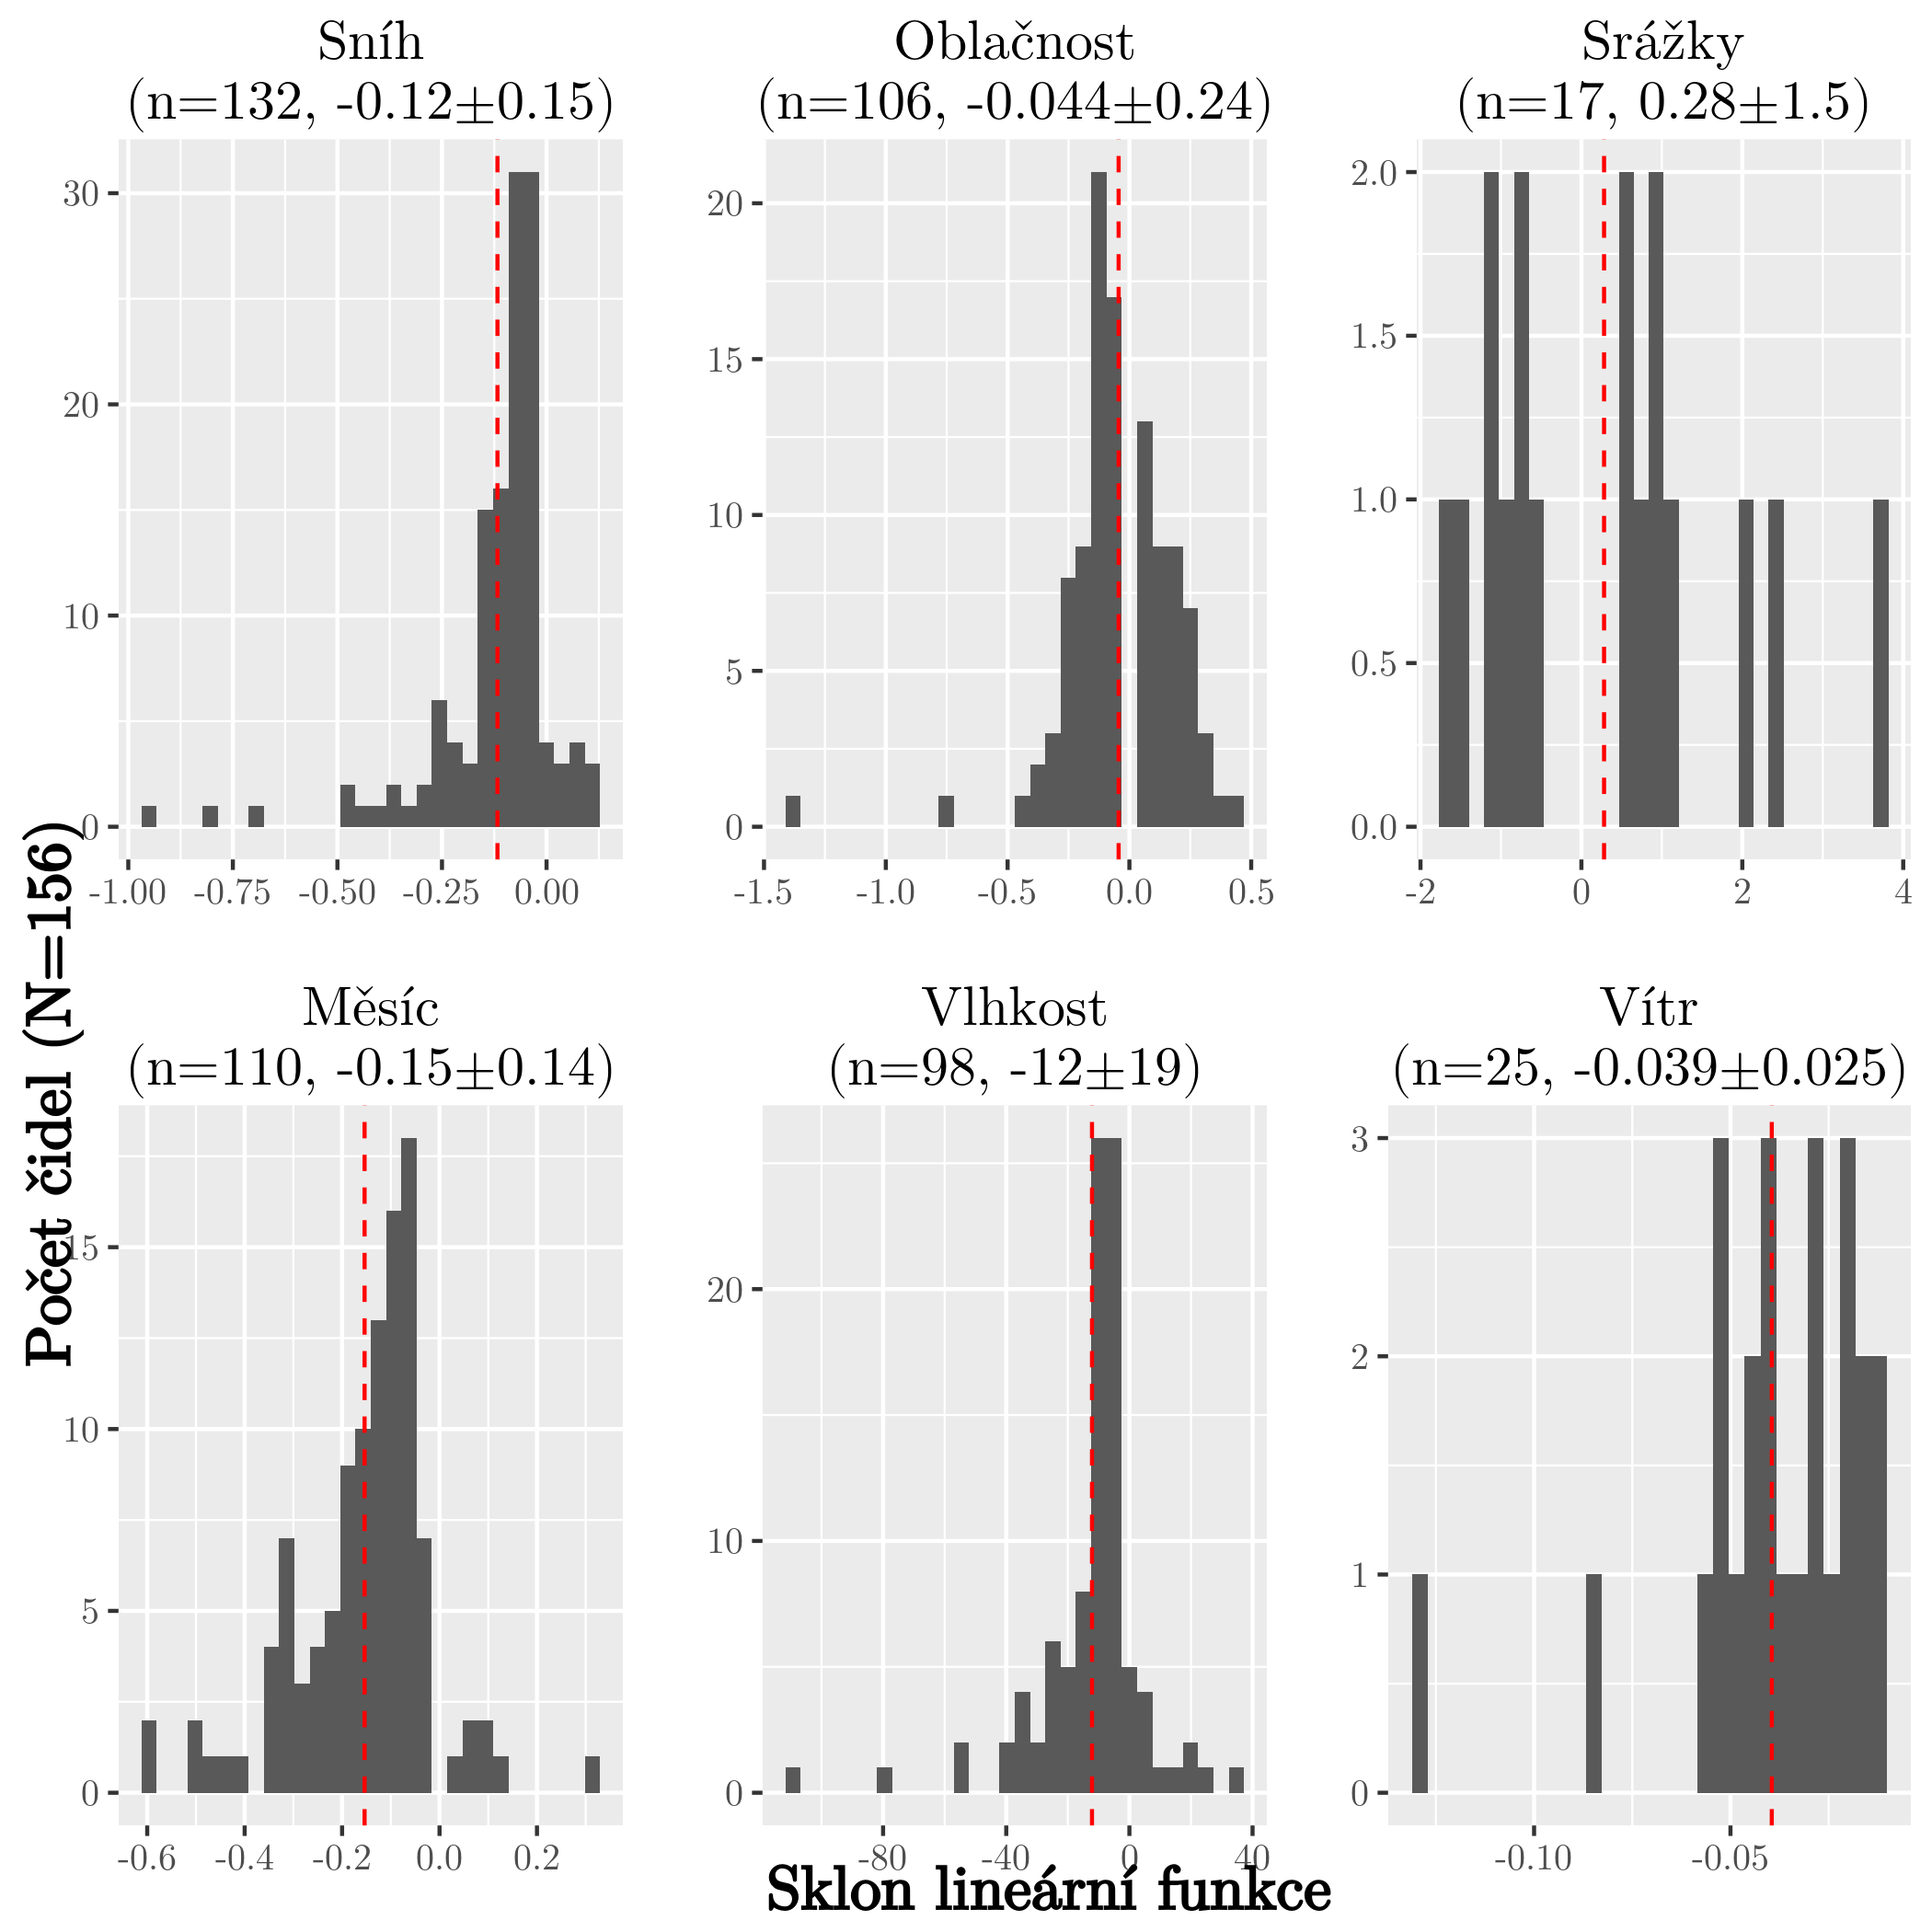
\includegraphics[width=0.8\linewidth,height=0.6\textwidth]{all156maxTall15cm_BWyes.png}
		\caption{Maximální denní teplota v $\SI{15}{cm}$}
	\end{figure}
\end{frame}

\begin{frame}
	\frametitle{Maximální teploty}
	\begin{itemize}
		\item Sníh: pro $\SI{15}{cm}$ má záporný vliv.
		\item Oblačnost: pro $\SI{0}{cm}$ má kladný vliv.
		\item Srážky: signifikantní pro málo čidel.
		\item Měsíc: záporný vliv.
		\item Vlhkost: záporný vliv.
		\item Vítr: záporný vliv (málo čidel).
	\end{itemize}
\end{frame}

\begin{frame}
	\frametitle{Minimální teploty}
	\begin{figure}
		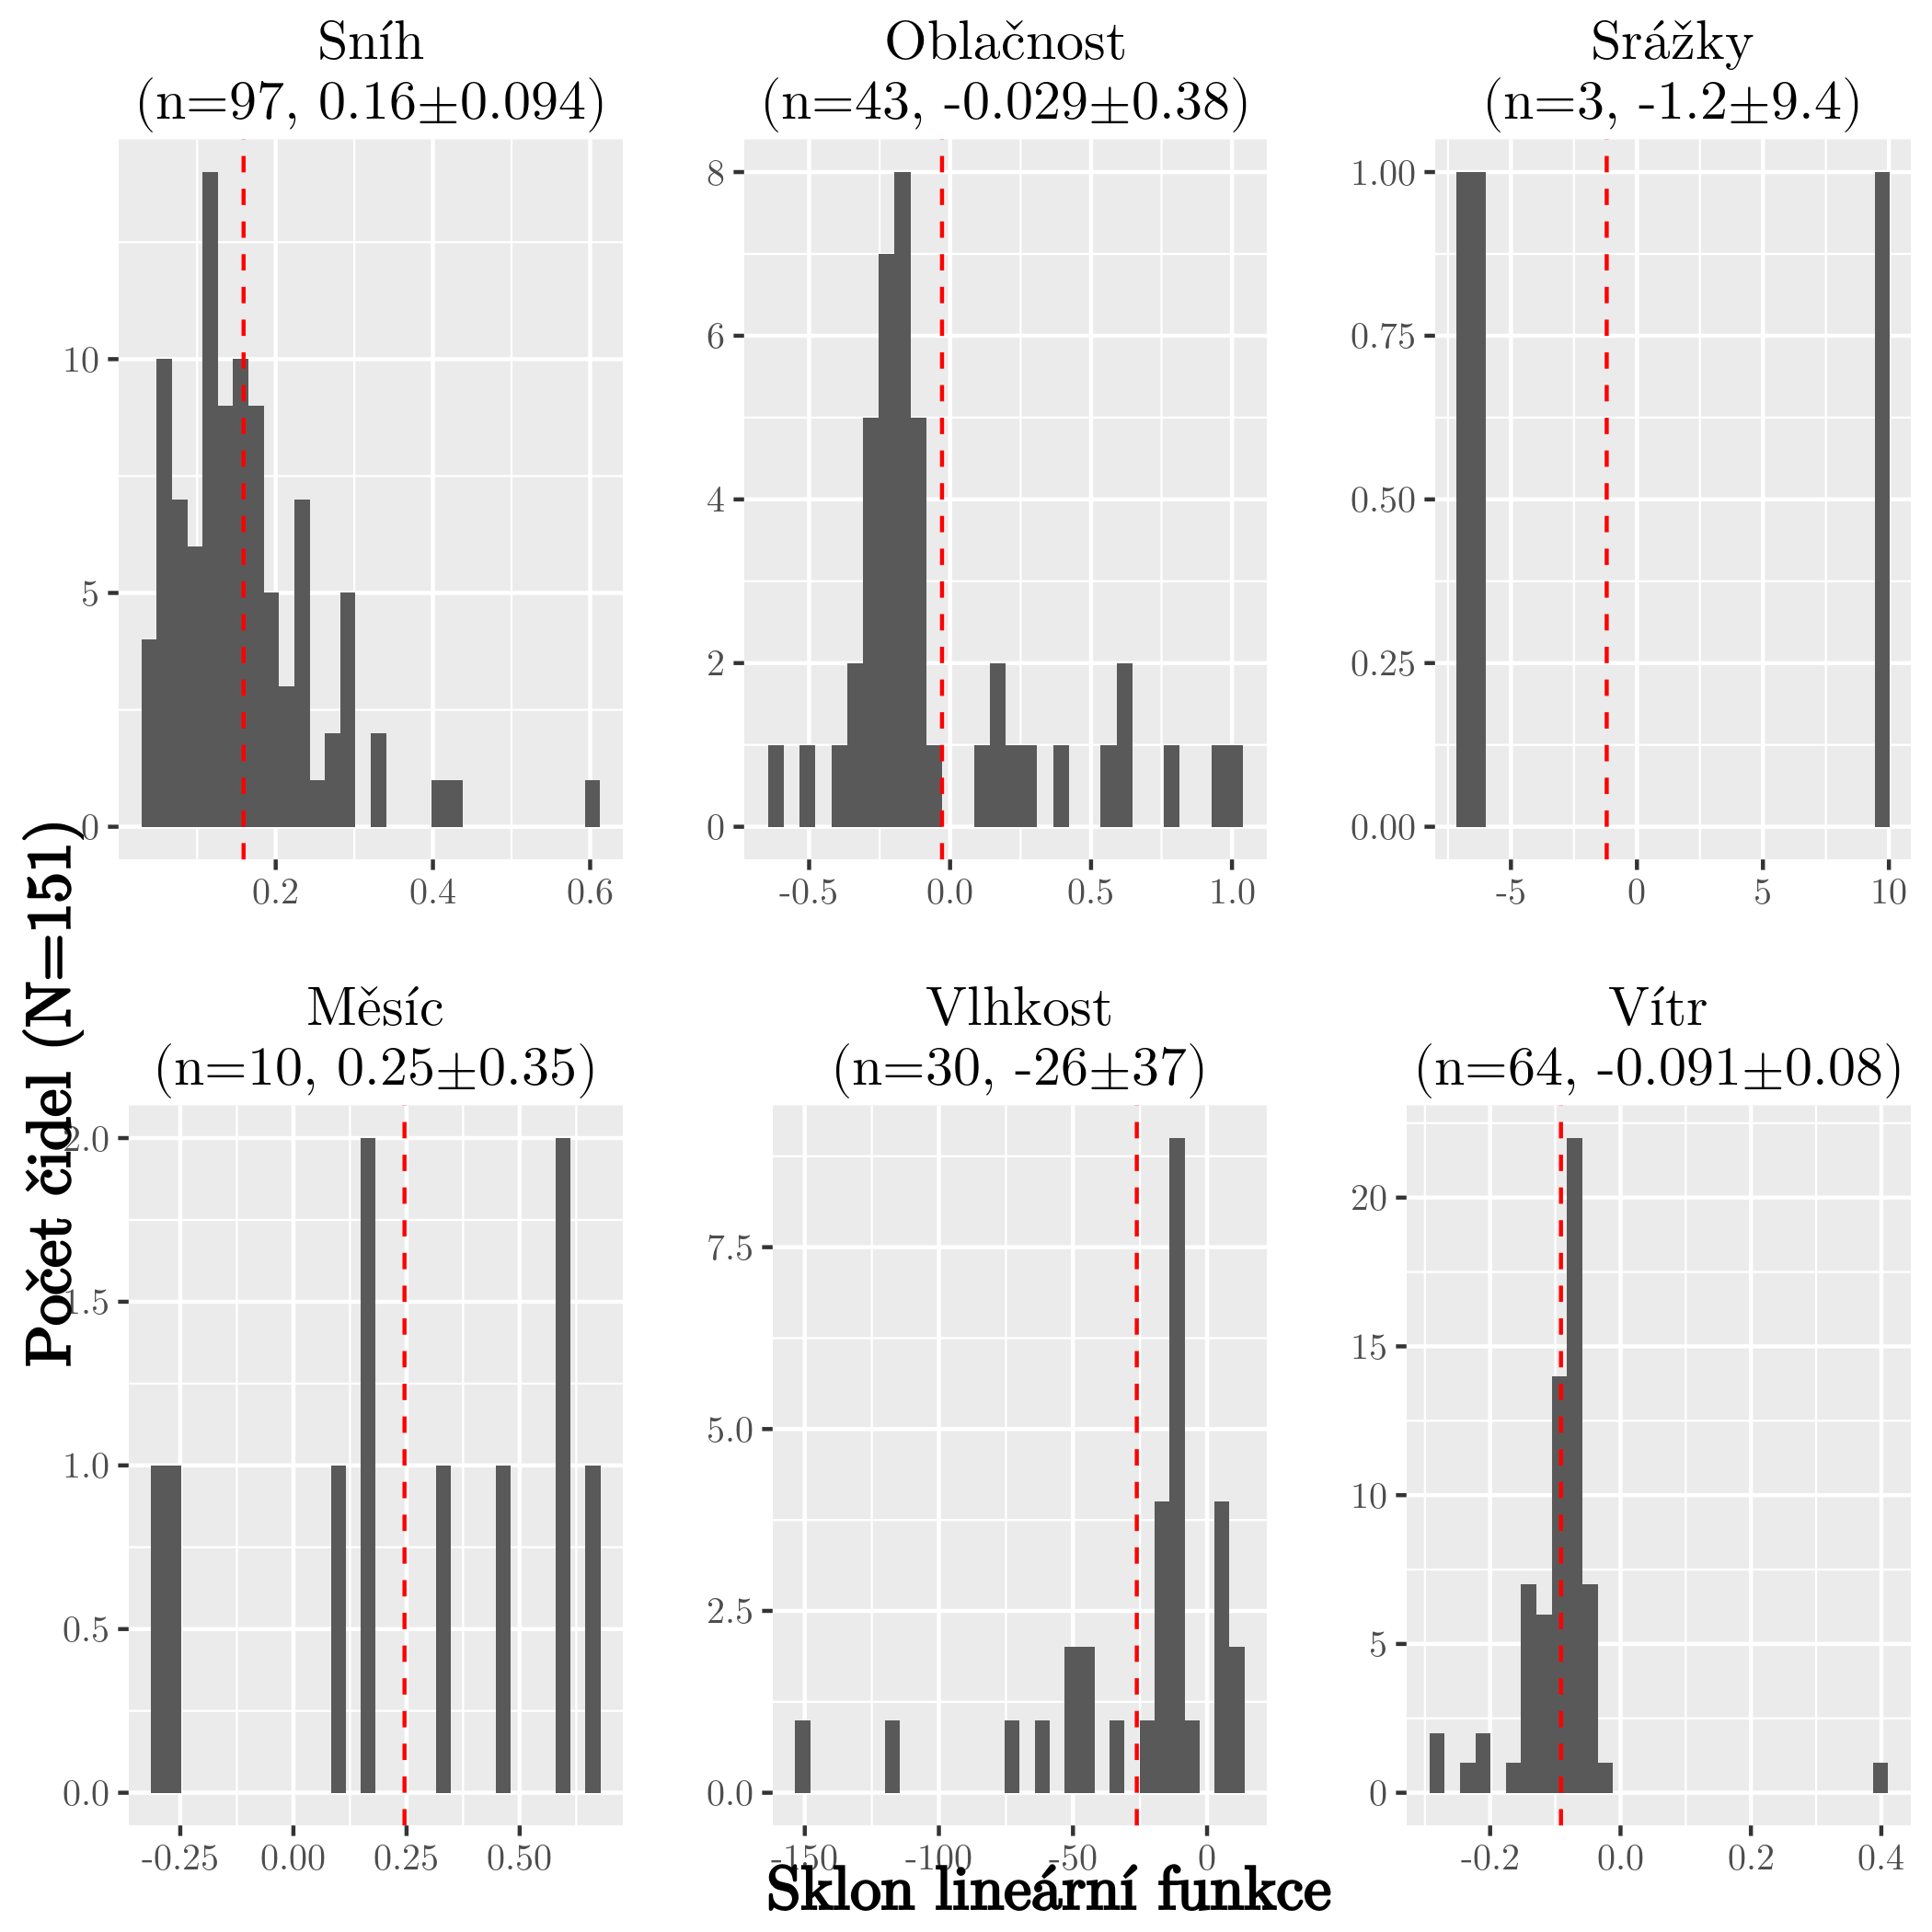
\includegraphics[width=0.8\linewidth,height=0.6\textwidth]{all151minTall0cm_BWyes.png}
		\caption{Minimální denní teplota v $\SI{0}{cm}$}
	\end{figure}
\end{frame}

\begin{frame}
	\frametitle{Minimální teploty}
	\begin{figure}
		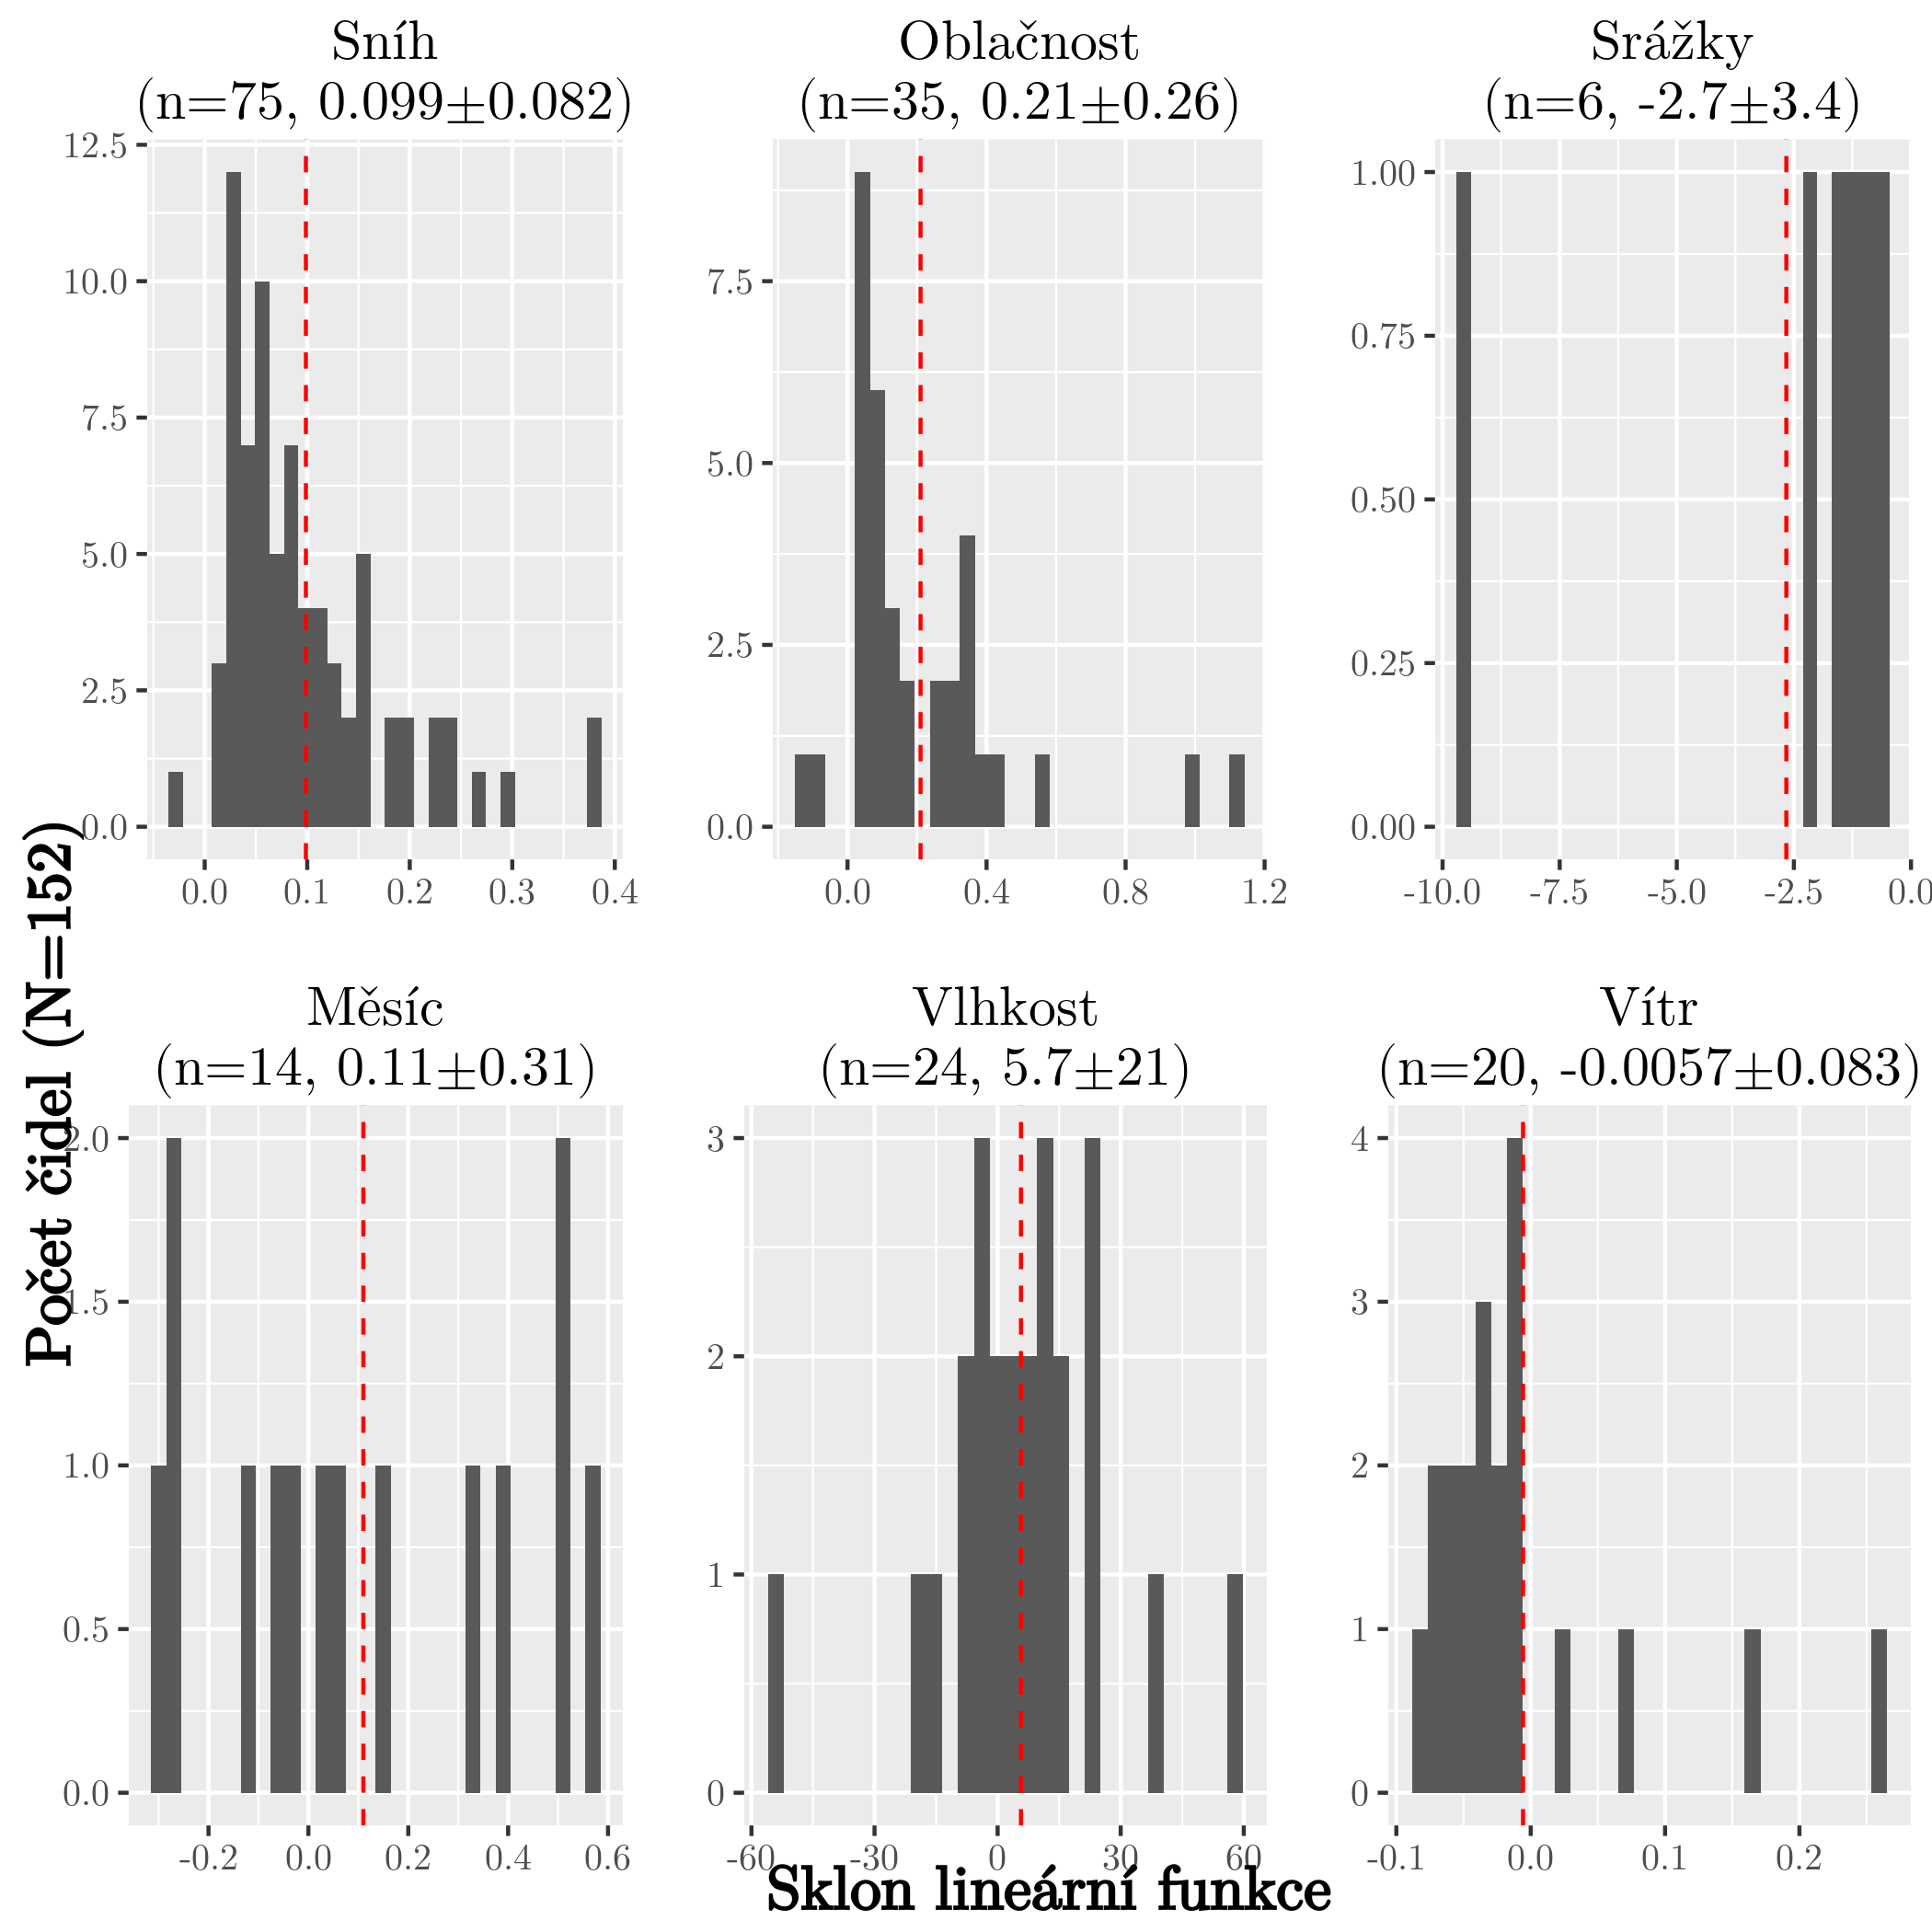
\includegraphics[width=0.8\linewidth,height=0.6\textwidth]{all152minTall15cm_BWyes.png}
		\caption{Minimální denní teplota v $\SI{15}{cm}$}
	\end{figure}
\end{frame}

\begin{frame}
	\frametitle{Minimální teploty}
	\begin{itemize}
		\item Sníh: kladný vliv.
		\item Oblačnost: pro $\SI{15}{cm}$ má kladný vliv.
		\item Srážky: signifikantní pro málo čidel.
		\item Měsíc: signifikantní pro málo čidel.
		\item Vlhkost: pro $\SI{0}{cm}$ má záporný vliv.
		\item Vítr: pro $\SI{0}{cm}$ má záporný vliv.
	\end{itemize}
\end{frame}
%------------------------------------------------

\section{Diskuze}

\begin{frame}
	\frametitle{Diskuze}
	\begin{itemize}
		\item Prediktor insolace místo měsíce?
		\item Sofistikovanější metody vyhodnocení?
	\end{itemize}
\end{frame}

%------------------------------------------------

%----------------------------------------------------------------------------------------
%	CLOSING SLIDE
%----------------------------------------------------------------------------------------

\begin{frame}[plain] % The optional argument 'plain' hides the headline and footline
	\begin{center}
		{\Huge Konec}
		
		\bigskip\bigskip % Vertical whitespace
		
		{\LARGE Otázky?}
	\end{center}
\end{frame}

%----------------------------------------------------------------------------------------

\end{document} 
